% presentation
\documentclass[compress]{beamer}

% handout
%\documentclass[handout]{beamer}

\usepackage{../mtex,fancyvrb,booktabs}
\usepackage{tikz}
%\usepackage{subfigure}
\usepackage[labelformat=empty]{subcaption}
\captionsetup{compatibility=false}

\author{R. Hielscher}

\title{Crystal Geometry}
%\subtitle{Chemnitz {\bf{\color{red}M}TEX} Workshop 2015}

\institute{Faculty of Mathematics,\\
	Chemnitz University of Technology, Germany}

\date{{\bf{\color{red}M}TEX} Workshop 2016}


\newcommand{\crystal}[5]{%
  \draw[->, >=latex, #5] (#1) --+ (#2);%
  \draw[->, >=latex, #5] (#1) --+ (#3);%
  \draw[->, >=latex, #5] (#1) --+ (#4);%
}

\newcommand{\fillcrystal}[5]{%
  \filldraw[fill=red!25,draw=red!35,opacity=0.5]
%  (0,0) + (1,0) -- (0,0) --++ (0,1) --+ (1,0);
  (#1) +(#2) -- (#1) --++ (#3) -- +(#2) ;%
  \filldraw[fill=red!45,draw=red!35,opacity=0.5]
  (#1) +(#3) -- (#1) --++ (#4) -- +(#3) ;%
  \filldraw[fill=red!65,draw=red!35,opacity=0.5]
  (#1) +(#4) -- (#1) --++ (#2) -- +(#4) ;%
  \draw[->, >=latex, #5] (#1) --+ (#2);%
  \draw[->, >=latex, #5] (#1) --+ (#3);%
  \draw[->, >=latex, #5] (#1) --+ (#4);%
}

\newcommand{\filldirection}[5]{%
  \filldraw[fill=red!25,draw=red!35,opacity=0.5]
%  (0,0) + (1,0) -- (0,0) --++ (0,1) --+ (1,0);
  (#1) +(#2) -- (#1) --++ (#3) -- +(#2) ;%
  \filldraw[fill=red!45,draw=red!35,opacity=0.5]
  (#1) +(#3) -- (#1) --++ (#4) -- +(#3) ;%
  \filldraw[fill=red!65,draw=red!35,opacity=0.5]
  (#1) +(#4) -- (#1) --++ (#2) -- +(#4) ;%
  \draw[->, >=latex, #5] (#1) --+ (#2);%
  \draw[->, >=latex, #5] (#1) --+ (#3);%
  \draw[->, >=latex,color=red, very thick] (#1) --+ (#4);%
}


\begin{document}

\begin{frame}
  \maketitle{}
\end{frame}

\begin{frame}
  \frametitle{Table of Content}

\tableofcontents{}

\end{frame}


\section{Vectors}

\subsection*{Vector3d}

\begin{frame}[fragile]
  \frametitle{Three dimensional vectors - The \MTEX Class \texttt{\bf vector3d}}

  \begin{overlayarea}{\textwidth}{8cm}
  Three dimensional vectors are given by there coordinates with respect to a
  orthogonal coordinate system $\vec X, \vec Y, \vec Z$
  \begin{equation*}
    \vec r = x \cdot \vec X + y \cdot \vec Y + z \cdot \vec Z
  \end{equation*}

  \pause

  For general vectors, MTEX does \textbf{not} care about the coordinate system, but
  works only with the coordinates.

  \begin{columns}
    \begin{column}{8cm}

      \begin{lstlisting}[style=input]
r = vector3d(1,2,3)
  \end{lstlisting}
      \begin{onlyenv}<2>
        \vspace{-0.3cm}
\begin{lstlisting}[style=output]
r = /+vector3d+/ (show methods, plot)
  size: 1 x 1
  x y z
  1 2 3
\end{lstlisting}
      \end{onlyenv}


      \pause
      \medskip

      The alignment of the coordinate system is only important when plotting
      data
      \begin{onlyenv}<3|handout>
\begin{lstlisting}[style=input]
plotx2north, plotzOutOfPlane
plot(r)
\end{lstlisting}
      \end{onlyenv}
      \begin{onlyenv}<4>
\begin{lstlisting}[style=input]
plotx2east, plotzOutOfPlane
plot(r)
\end{lstlisting}
      \end{onlyenv}

    \end{column}
    \begin{column}{3.5cm}
      \only<3|handout>{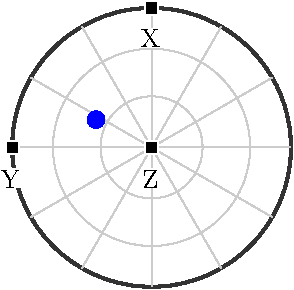
\includegraphics[width=3.5cm]{pic/vectorNorth}}
      \only<4>{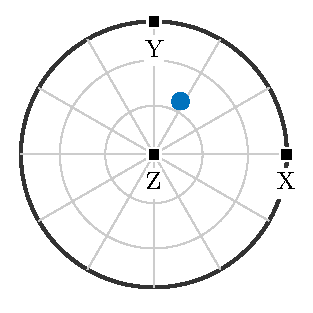
\includegraphics[width=3.5cm]{pic/vectorEast}}
    \end{column}
  \end{columns}

  \pause
  \medskip

  Only for directions relative to the crystal coordinate system the reference
  frame is considered.

\end{overlayarea}
\end{frame}

\subsection*{Definition}

\begin{frame}[fragile,fragile,fragile]
  \frametitle{Defining vectors}

  \begin{overlayarea}{\textwidth}{8cm}

    polar coordinates $\vec r = (\sin \theta \cos \rho,\sin \theta \sin \rho,\cos \theta)^{t}$

\begin{lstlisting}[style=input]
r = vector3d('theta',theta,'rho',rho)
\end{lstlisting}

  \pause \medskip

  predefined vectors
\begin{lstlisting}[style=input]
vector3d.X, vector3d.Y, vector3d.Z
\end{lstlisting}

  \pause \medskip

  combine vectors
\begin{lstlisting}[style=input]
r = [vector3d.X, vector3d.Y, vector3d(1,1,1)];
\end{lstlisting}

\begin{onlyenv}<3>
  \vspace{-.3cm}
\begin{lstlisting}[style=output]
r = /+vector3d+/ (show methods, plot)
  size: 1 x 3
  x y z
  1 0 0
  0 1 0
  1 1 1
\end{lstlisting}
\end{onlyenv}
  \pause \medskip

  importing vectors
\begin{lstlisting}[style=input]
r = loadVector3d('file','ColumnNames',{'x','y','z'})
\end{lstlisting}
\begin{onlyenv}<4>
  \vspace{-.3cm}
\begin{lstlisting}[style=output]
r = /+vector3d+/ (show methods, plot)
  size: 200 x 1
\end{lstlisting}
\end{onlyenv}

\end{overlayarea}
\end{frame}

\subsection*{Calculations}

\begin{frame}[fragile]
  \frametitle{Vector Calculations}

  simple algebra
\begin{lstlisting}[style=input]
r = 2*vector3d.X - vector3d.Y;
\end{lstlisting}

  \pause \medskip


  basic operations
\begin{lstlisting}[style=input]
dot(v1,v2)   % dot product
cross(v1,v2) % cross product
angle(v1,v2) % angle between two vectors
\end{lstlisting}

  \pause \medskip

  extract properties
\begin{lstlisting}[style=input]
r.theta      % polar angle in radiant
r.rho        % azimuth angle in radiant
r.x, r.y, r.z
\end{lstlisting}

\end{frame}


\subsection*{Indexing}

\begin{frame}[fragile]
  \frametitle{Indexing of Vectors}

  \begin{overlayarea}{\textwidth}{8cm}

    consider a list of vectors
    \begin{lstlisting}[style=input]
r = vector3d([0 0 1 1],[1 0 1 1],[1 1 1 0]);
    \end{lstlisting}

    \begin{onlyenv}<1>
      \vspace{-.3cm}
      \begin{lstlisting}[style=output]
r = /+vector3d+/ (show methods, plot)
  size: 1 x 4
  x y z
  0 1 1
  0 0 1
  1 1 1
  1 1 0
      \end{lstlisting}
    \end{onlyenv}

    \pause \medskip

    single out the second vector
    \begin{lstlisting}[style=input]
r(2)
    \end{lstlisting}

    \begin{onlyenv}<2>
      \vspace{-0.3cm}
      \begin{lstlisting}[style=output]
r = /+vector3d+/ (show methods, plot)
  size: 1 x 1
  x y z
  0 0 1
      \end{lstlisting}
    \end{onlyenv}

    \pause \medskip

    single out the second and the fourth vector
    \begin{lstlisting}[style=input]
r([2 4])
    \end{lstlisting}
    \begin{onlyenv}<3>
      \vspace{-0.3cm}
      \begin{lstlisting}[style=output]
r = /+vector3d+/ (show methods, plot)
  size: 1 x 2
  x y z
  0 0 1
  1 1 0
      \end{lstlisting}
    \end{onlyenv}

  \pause \medskip

single out vectors by a logical condition
    \begin{lstlisting}[style=input]
r(r.x>0)
    \end{lstlisting}
        \begin{onlyenv}<4>
          \vspace{-0.3cm}
      \begin{lstlisting}[style=output]
r = /+vector3d+/ (show methods, plot)
  size: 1 x 2
  x y z
  1 1 1
  1 1 0
     \end{lstlisting}
    \end{onlyenv}

    \pause \medskip

    \alert{The above techniques applies also to lists of rotations,
      orientations, tensors, EBSD data, grains, boundary segments, triple
      points, etc.}
  \end{overlayarea}
\end{frame}


\subsection*{Changing Vectors}

\begin{frame}[fragile]
  \frametitle{Changing Vectors}

  \begin{overlayarea}{\textwidth}{8cm}

    consider again the list of vectors
    \begin{lstlisting}[style=input]
r = vector3d([0 0 1 1],[1 0 1 1],[1 1 1 0]);
    \end{lstlisting}

    \begin{onlyenv}<1>
      \vspace{-0.3cm}
      \begin{lstlisting}[style=output]
r = /+vector3d+/ (show methods, plot)
  size: 1 x 4
  x y z
  0 1 1
  0 0 1
  1 1 1
  1 1 0
      \end{lstlisting}
    \end{onlyenv}

    \pause \medskip

    replace the second vector by another vector
    \begin{lstlisting}[style=input]
r(2) = vector3d.Y
    \end{lstlisting}

    \begin{onlyenv}<2>
      \vspace{-0.3cm}
      \begin{lstlisting}[style=output]
r = /+vector3d+/ (show methods, plot)
  size: 1 x 4
  x y z
  0 1 1
  0 1 0
  1 1 1
  1 1 0
      \end{lstlisting}
    \end{onlyenv}

    \pause \medskip

    remove the second vector completely
    \begin{lstlisting}[style=input]
r(2) = []
    \end{lstlisting}
    \begin{onlyenv}<3>
      \vspace{-0.3cm}
      \begin{lstlisting}[style=output]
r = /+vector3d+/ (show methods, plot)
  size: 1 x 3
  0 1 1
  1 1 1
  1 1 0
      \end{lstlisting}
    \end{onlyenv}

  \pause \medskip

  change the x coordinate of all vectors
    \begin{lstlisting}[style=input]
r.x = 0
    \end{lstlisting}
        \begin{onlyenv}<4>
          \vspace{-0.3cm}
      \begin{lstlisting}[style=output]
r = /+vector3d+/ (show methods, plot)
  size: 1 x 3
  0 1 1
  0 1 1
  0 1 0
     \end{lstlisting}
    \end{onlyenv}

    \pause \medskip

    \alert{The above techniques applies also to pole figure data,
    orientations, EBSD data, grains, etc.}
  \end{overlayarea}


\end{frame}


\subsection*{Plotting}
\label{sec:plotting}

\begin{frame}[fragile]
  \frametitle{Plotting Vectors}

  \begin{columns}
    \begin{column}{8.6cm}
      \begin{overlayarea}{\textwidth}{8cm}

      spherical projections: \texttt{earea, edist, eangle}
      %hemisphere: \texttt{upper, lower}

      \begin{onlyenv}<1>
        \begin{lstlisting}[style=input]
plot(r,'projection','eangle','upper')
\end{lstlisting}
      \end{onlyenv}

      \pause

      \begin{onlyenv}<2->
        \begin{lstlisting}[style=input]
plot(r,'projection','earea','upper')
\end{lstlisting}
      \end{onlyenv}

\pause \medskip

combined plots
\vspace{-0.1cm}
\begin{lstlisting}[style=input]
plot(vector3d(1,1,1),'upper');
hold all
plot(vector3d(1,2,3),'label','B');
plot(vector3d(-1,2,1),'label','A');
hold off
\end{lstlisting}

      \pause \medskip

      scatter plots
\vspace{-0.1cm}
      \begin{lstlisting}[style=input]
v = vector3d.rand(1000)
plot(v)
\end{lstlisting}
\pause
contour plots
\vspace{-0.1cm}
      \begin{lstlisting}[style=input]
plot(v,'contourf')
\end{lstlisting}

    \end{overlayarea}
  \end{column}

  \begin{column}{3.5cm}

    \begin{overlayarea}{\textwidth}{8cm}
      \includegraphics<1-2>[width=3.5cm]{pic/vectoreangle}

      \includegraphics<2>[width=3.5cm]{pic/vectorearea}

      \includegraphics<3>[width=3.5cm]{pic/vectorCombined}

      \includegraphics<4>[width=3.5cm]{pic/vectorScatter}

      \includegraphics<5>[width=3.5cm]{pic/vectorContour}
    \end{overlayarea}
  \end{column}
  \end{columns}

\end{frame}


\subsection*{data plots}

\begin{frame}[fragile]
  \frametitle{Data Plots}

  \begin{columns}
    \begin{column}{0.7\textwidth}
      colorize vectors by value
      \begin{lstlisting}[style=input]
v = vector3d.rand(100)
scatter(v,v.rho./degree,'upper',...
        'grid','on','minmax')
mtexColorbar('southoutside')
mtexColorMap jet
      \end{lstlisting}

      \pause

      colorize by RGB triples
      \begin{lstlisting}[style=input]
oM = ipdfHSVOrientationMapping
scatter(v,oM.Miller2color(v))
      \end{lstlisting}

      \pause

      visualize directions
      \begin{lstlisting}[style=input]
quiver(v,orth(v)) % a vector field
      \end{lstlisting}

    \end{column}
    \begin{column}{0.3\textwidth}
      \begin{overlayarea}{\textwidth}{8cm}
        \includegraphics<1-2>[width=\textwidth]{pic/vectorColor}

        \includegraphics<2>[width=\textwidth]{pic/vectorRGBColor}

        \includegraphics<3>[width=\textwidth]{pic/quiver}
    \end{overlayarea}
    \end{column}
  \end{columns}

\end{frame}

\subsection*{Annotations}

\begin{frame}[fragile]
  \frametitle{Customize Plots}

\begin{columns}
  \begin{column}{8.5cm}

\begin{overprint}
  \onslide<1|handout:0>%
  General Syntax%
\begin{lstlisting}[style=input]
plot(vector3d,<options>)
\end{lstlisting}
  \onslide<2|handout:1>%
  General Syntax
\begin{lstlisting}[style=input]
annotate(orientation,<options>)
\end{lstlisting}
\end{overprint}

Options
\begin{lstlisting}[style=input]
Marker            % marker shape
MarkerSize        % marker size
MarkerFaceColor   % face color
MarkerEdgeColor   % edge color
label             % a label text
color, background % text colors
\end{lstlisting}

\begin{overprint}
  \onslide<1|handout:0>%
  Example
\begin{lstlisting}[style=input]
plot([vector3d.X,vector3d.Y,vector3d.Z],
 'Backgroundcolor','w','Marker','s',
 'MarkerEdgeColor','w','labeled',
 'MarkerFaceColor','k')
\end{lstlisting}

  \onslide<2|handout:1>
Example
\begin{lstlisting}[style=input]
plot(q0,'label','A',...
 'Backgroundcolor','w','Marker','s',
 'MarkerEdgeColor','w',...
 'MarkerFaceColor','r')
\end{lstlisting}

\end{overprint}

\end{column}

\begin{column}{3.5cm}
    \onslide<1->
    \only<1|handout:0>{%
    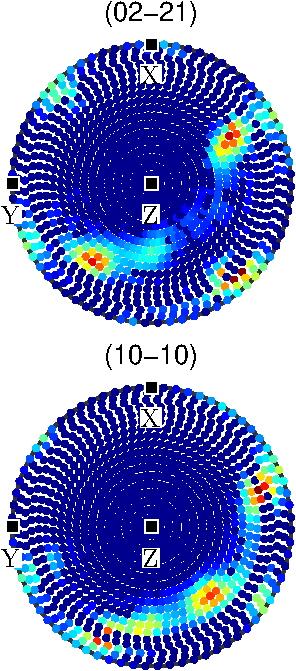
\includegraphics[width=3.5cm]{pic/annotationv}%
    }%
    \only<2>{%
    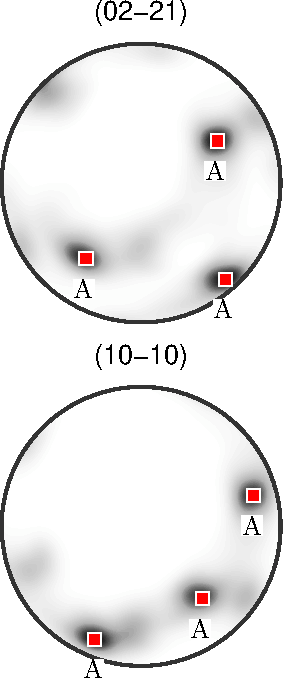
\includegraphics[width=3.3cm]{pic/annotationq}%
    }%
\end{column}

\end{columns}

\end{frame}

\subsection*{Axes}

\begin{frame}[fragile]
  \frametitle{Axes}

  \begin{columns}
    \begin{column}{8.5cm}
      \begin{overlayarea}{8.5cm}{8cm}
        Axes are three dimensional vectors where we do not care about length and
        direction, e.g. plane normals.

\begin{lstlisting}[style=input]
r = vector3d(1,1,1,'antipodal')
\end{lstlisting}

\medskip
\pause

Then \textbf{\texttt{r}} and \textbf{\texttt{-r}} represent the same axis
\begin{lstlisting}[style=input]
eq(r, -r)
\end{lstlisting}
\begin{onlyenv}<2>
  \vspace{-0.3cm}
\begin{lstlisting}[style=output]
  1
\end{lstlisting}
\end{onlyenv}

\medskip
\pause

The angle to an axis is always less then $90^{\degree}$
\begin{lstlisting}[style=input]
angle(r,-vector3d.X) / degree
\end{lstlisting}
\begin{onlyenv}<3>
  \vspace{-0.3cm}
\begin{lstlisting}[style=output]
  54.7
\end{lstlisting}
\end{onlyenv}

\medskip
\pause

The option \textbf{antipodal} in a contour plot
\begin{onlyenv}<4>
\begin{lstlisting}[style=input]
r = vector3d.rand(1000)
plot(r,'contourf')
\end{lstlisting}
\end{onlyenv}
\begin{onlyenv}<5>
\begin{lstlisting}[style=input]
r = randv(1000)
plot(r,'contourf','antipodal')
\end{lstlisting}
\end{onlyenv}
\end{overlayarea}
\end{column}
  \begin{column}{3.5cm}
    \only<1-3>{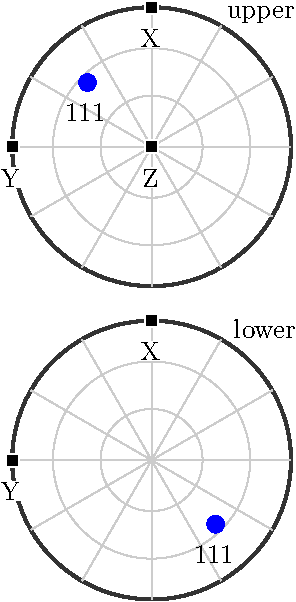
\includegraphics[width=3.5cm]{pic/vectorAntipodal}}
    \only<4>{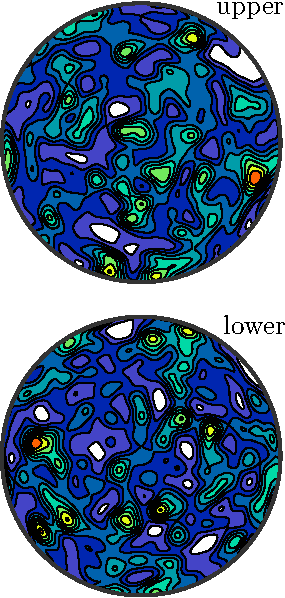
\includegraphics[width=3.5cm]{pic/vectorContour}}
    \only<5>{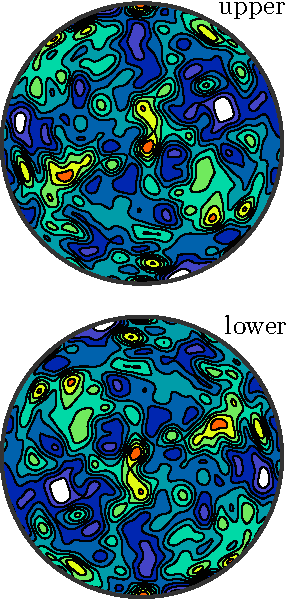
\includegraphics[width=3.5cm]{pic/vectorContourAntipodal}}
  \end{column}
\end{columns}


\end{frame}

\section{Rotations}

\subsection*{Basics}

\begin{frame}[fragile]
  \frametitle{Rotations}

  A rotation is a transformation that maps a right handed coordinate system
  $(\vec X_{1}, \vec Y_{1}, \vec Z_{1})$ onto another right handed coordinate
  system $(\vec X_{2}, \vec Y_{2}, \vec Z_{2})$. It is given by the rotation
  matrix

  % \begin{equation*}
  %   \bf R = \left(
  %     \begin{matrix}
  %       \vec X_{1} \cdot \vec X_{2} & \vec Y_{1} \cdot \vec X_{2}& \vec Z_{1} \cdot \vec X_{2} \\
  %       \vec X_{1} \cdot \vec Y_{2} & \vec Y_{1} \cdot \vec Y_{2}& \vec Z_{1} \cdot \vec Y_{2} \\
  %       \vec X_{1} \cdot \vec Z_{2} & \vec Y_{1} \cdot \vec Z_{2}& \vec Z_{1} \cdot \vec Z_{2}
  %     \end{matrix}
  %   \right).
  % \end{equation*}
  \begin{equation*}
    \mathbf R = (\vec X_{2}, \vec Y_{2}, \vec Z_{2}) \cdot (\vec X_{1}, \vec Y_{1}, \vec Z_{1})^{t}
  \end{equation*}

  \medskip

  We have $\mathbf R \vec X_{1} = \vec X_{2}$, $\mathbf R \vec Y_{1} = \vec
  Y_{2}$ and $\mathbf R \vec Z_{1} = \vec Z_{2}$.

  \medskip
  \pause

  On the other hand, $\bf R$ transforms coordinates with respect to $(\vec
  X_{2}, \vec Y_{2}, \vec Z_{2})$ into coordinates with respect to $(\vec
  X_{1}, \vec Y_{1}, \vec Z_{1})$. I.e. for

  \begin{equation*}
    \vec r
    = x_{1} \vec X_{1} + y_{1} \vec Y_{1} + z_{1} \vec Z_{1}
    = x_{2} \vec X_{2} + y_{2} \vec Y_{2} + z_{2} \vec Z_{2}
  \end{equation*}

  we have

  \begin{equation*}
    \mathbf R
    \left(
      \begin{matrix}
        x_{2}\\
        y_{2}\\
        z_{2}
      \end{matrix}\right)
    = \left(
      \begin{matrix}
        x_{1}\\
        y_{1}\\
        z_{1}
      \end{matrix}\right)
  \end{equation*}

\end{frame}

\subsection*{Euler Angles}
\label{sec:euler-angles}

\begin{frame}[fragile]
  \frametitle{Euler Angles}
  \begin{overlayarea}{\textwidth}{8cm}

  Most commonly, rotations are given by Bunge Euler angles.

  \begin{lstlisting}[style=input]
R = rotation('Euler',10*degree,20*degree,30*degree)
  \end{lstlisting}
  \begin{onlyenv}<1>
    \vspace{-0.3cm}
  \begin{lstlisting}[style=output]
R = /+rotation+/ (show methods, plot)
  size: 1 x 1

  Bunge Euler angles in degree
  phi1  Phi phi2 Inv.
    10   20   30    0
  \end{lstlisting}
  \end{onlyenv}

  \pause
  \medskip

  \begin{lstlisting}[style=input]
R = rotation('Euler',...
    10*degree,20*degree,30*degree,'Roe')
  \end{lstlisting}
  \begin{onlyenv}<2>
    \vspace{-0.3cm}
  \begin{lstlisting}[style=output]
R = /+rotation+/ (show methods, plot)
  size: 1 x 1

  Bunge Euler angles in degree
  phi1  Phi phi2 Inv.
   100   20  300    0
  \end{lstlisting}
\end{onlyenv}

\pause
\medskip

Supported conventions are \texttt{Bunge}, \texttt{Matthies}, \texttt{Roe},
\texttt{Kocks}, \texttt{Canova}.
  \begin{lstlisting}[style=input]
setMTEXpref('EulerAngleConvention','Roe')
  \end{lstlisting}

  \begin{onlyenv}<3>
    \vspace{-0.3cm}
  \begin{lstlisting}[style=output]
R = /+rotation+/ (show methods, plot)
  size: 1 x 1

  Roe Euler angles in degree
  Psi Theta   Phi Inv.
   10    20    30    0
 \end{lstlisting}
\end{onlyenv}
\end{overlayarea}
\end{frame}

\subsection*{Axis Angle Representation}
\label{sec:axis-angle-repr}

\begin{frame}[fragile]
  \frametitle{Other Ways to Define a Rotation}

  A rotation is uniquely defined by its rotation axis and its rotation angle

  \begin{lstlisting}[style=input]
R = rotation('axis',vector3d.X,'angle',45*degree)
  \end{lstlisting}

  \pause
  \medskip

  Conversely, one can compute axis / angle from a rotation

  \begin{lstlisting}[style=input]
R.axis, R.angle
  \end{lstlisting}

  \pause
  \medskip

Given four vectors $\vec u_{1}, \vec u_{2}, \vec v_{1}, \vec v_{2}$ there is a
unique rotation $\mathbf R$ such that  $\mathbf R \vec u_{1} = \vec v_{1}$ and
$\mathbf R \vec u_{2} = \vec v_{2}$

\begin{lstlisting}[style=input]
R = rotation('map',u1,v1,u2,v2)
\end{lstlisting}

  \pause
  \medskip

Of course one can also define a rotation by its $3 \times 3$ matrix

  \begin{lstlisting}[style=input]
R = rotation('matrix',A)
  \end{lstlisting}

or by quaternions

  \begin{lstlisting}[style=input]
R = rotation('quaternion',a,b,c,d)
  \end{lstlisting}

\end{frame}

\subsection*{Basic Calculations}
\label{sec:euler-angles}

\begin{frame}[fragile]
  \frametitle{Basic Calculations}

    rotate a vector
    \begin{lstlisting}[style=input]
R = rotation('axis',vector3d.X,'angle',-45*degree);
R * vector3d(0,1,1)
    \end{lstlisting}


  \begin{columns}
    \begin{column}{8cm}
  \begin{overlayarea}{8cm}{8cm}
\begin{onlyenv}<1>
  \vspace{-0.3cm}
\begin{lstlisting}[style=output]
ans = /+vector3d+/ (show methods, plot)
  size: 1 x 1
  x       y       z
  0 1.41421       0
  \end{lstlisting}
\end{onlyenv}

\pause
 \medskip

 the inverse rotation
 \begin{lstlisting}[style=input]
 inv(R)
 \end{lstlisting}
 \begin{onlyenv}<2>
   \vspace{-0.3cm}
  \begin{lstlisting}[style=output]
ans = /+rotation+/ (show methods, plot)
  size: 1 x 1

  Bunge Euler angles in degree
  phi1  Phi phi2 Inv.
     0   45    0    0
  \end{lstlisting}
 \end{onlyenv}

 \pause
 \medskip

 combine rotations
 \begin{lstlisting}[style=input]
R * inv(R)
\end{lstlisting}

\begin{onlyenv}<3>
  \vspace{-0.3cm}
  \begin{lstlisting}[style=output]
ans = /+rotation+/ (show methods, plot)
  size: 1 x 1

  Bunge Euler angles in degree
  phi1  Phi phi2 Inv.
     0    0    0    0
  \end{lstlisting}
\end{onlyenv}

\pause
\medskip

plotting
\begin{lstlisting}[style=input]
R = rotation.rand(100)
scatter(R)      % axis angle plot
\end{lstlisting}

\end{overlayarea}
\end{column}

\begin{column}{3.7cm}
  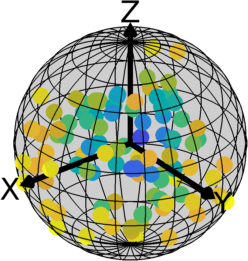
\includegraphics[width=3.7cm]{pic/rotationScatter.png}
\end{column}

\end{columns}

\end{frame}

\subsection*{Improper Rotations}

\begin{frame}[fragile]
  \frametitle{Improper Rotations}

  \begin{overlayarea}{\textwidth}{7cm}

    An improper rotation is a rotation followed by an inversion
    \begin{lstlisting}[style=input]
I = -rotation('Euler',10*degree,20*degree,30*degree)
    \end{lstlisting}
    \begin{onlyenv}<1>
      \vspace{-0.3cm}
      \begin{lstlisting}[style=output]
I = /+rotation+/ (show methods, plot)
  size: 1 x 1

  Bunge Euler angles in degree
  phi1  Phi phi2 Inv.
    10   20   30    1
  \end{lstlisting}
  \end{onlyenv}

  \pause
  \bigskip

  reflections
  \begin{lstlisting}[style=input]
R = reflection(vector3d.X + vector3d.Y)
  \end{lstlisting}
  \begin{onlyenv}<2>
    \vspace{-0.3cm}
  \begin{lstlisting}[style=output]
R = /+rotation+/ (show methods, plot)
  size: 1 x 1

  Bunge Euler angles in degree
  phi1  Phi phi2 Inv.
    45  180  315    1
  \end{lstlisting}
  \end{onlyenv}

  \pause
  \bigskip

  angles between proper and improper rotations
  \begin{lstlisting}[style=input]
angle(I,[R,-R])
  \end{lstlisting}
  \begin{onlyenv}<3>
    \vspace{-0.3cm}
    \begin{lstlisting}[style=output]
  168.5677  180.0000
  \end{lstlisting}
  \end{onlyenv}

  \pause
  \bigskip

  check for improper rotations
\begin{lstlisting}[style=input]
I.isImproper
  \end{lstlisting}
  \begin{onlyenv}<4>
    \vspace{-0.3cm}
    \begin{lstlisting}[style=output]
  1
  \end{lstlisting}
  \end{onlyenv}

\end{overlayarea}
\end{frame}

\section{Crystal Symmetries}
\label{sec:symmetries}

\subsection*{Crystal Symmetries}
\label{sec:crystal-symmetries}

\begin{frame}[fragile,fragile]
  \frametitle{Crystal Symmetry}

  \begin{columns}
  \begin{column}{8cm}

    \begin{overlayarea}{8cm}{8cm}
      The \alert{point group} $\mathbf C$ of a crystal are all rotations
      $\mathbf R$ that keep the crystal lattice invariant.

\begin{lstlisting}[style=input]
CS = crystalSymmetry('m-3m')
\end{lstlisting}
    \begin{onlyenv}<1>
\vspace{-.3cm}\begin{lstlisting}[style=output]
CS = /+crystalSymmetry+/ (show methods, plot)

  symmetry: m-3m
  a, b, c : 1, 1, 1
\end{lstlisting}
    \end{onlyenv}

    \pause \medskip

    extract the rotations of a point group
\begin{lstlisting}[style=input]
 rotation(crystalSymmetry('222'))
\end{lstlisting}
    \begin{onlyenv}<2>
\vspace{-.3cm}\begin{lstlisting}[style=output]
ans = /+rotation+/ (show methods, plot)
  size: 4 x 1

  Bunge Euler angles in degree
  phi1  Phi phi2 Inv.
     0    0    0    0
   180    0    0    0
    45  180   45    0
    45  180  225    0
\end{lstlisting}
    \end{onlyenv}

    \pause \medskip

    import data from crystal information files
\begin{lstlisting}[style=input]
CS = loadCIF('Quarz.cif')
\end{lstlisting}
    \begin{onlyenv}<3>
\vspace{-.3cm}\begin{lstlisting}[style=output]
CS = /+crystalSymmetry+/ (show methods, plot)

  mineral           : Quartz
  symmetry          : P 32 2 1 (321)
  a, b, c           : 4.9, 4.9, 5.4
  alpha, beta, gamma: 90°, 90°, 120°
  reference frame   : X||a*, Y||b, Z||c*
\end{lstlisting}
\end{onlyenv}

    \pause
    \vspace{-.3cm}

\begin{lstlisting}[style=input]
CS = loadPHL('minerals.phl')
\end{lstlisting}
    \begin{onlyenv}<4>
\vspace{-.3cm}\begin{lstlisting}[style=output]
CS{1} = /+crystalSymmetry+/ (show methods, plot)

  mineral : Magnetite
  density : 5.054
  symmetry: m-3m
  a, b, c : 8.4, 8.4, 8.4
\end{lstlisting}
\end{onlyenv}

\pause
\medskip

    switch to Laue / purely rotational group
\begin{lstlisting}[style=input]
CS.Laue
CS.properGroup
\end{lstlisting}

  \end{overlayarea}
\end{column}
  \begin{column}{3.7cm}
    \includegraphics<1->[width=3.7cm]{pic/m-3m}

    \medskip

    \includegraphics<3->[width=3.7cm]{pic/quartz}

    %\includegraphics<1-2>[width=3.7cm]{pic/m-3mHKL}
    %\includegraphics<3>[width=3.7cm]{pic/quartzHKL}
  \end{column}
\end{columns}
\end{frame}

\subsection*{Laue and Proper Symmetry Groups}
\begin{frame}[fragile]

  \begin{figure}[H]
    \centering
    \begin{subfigure}{0.3\textwidth}
      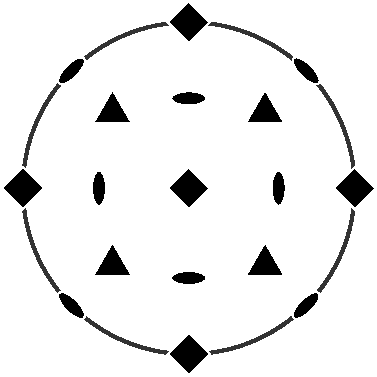
\includegraphics[width=\textwidth]{pic/432}
      \subcaption{$432$}
    \end{subfigure}
    \begin{subfigure}{0.3\textwidth}
      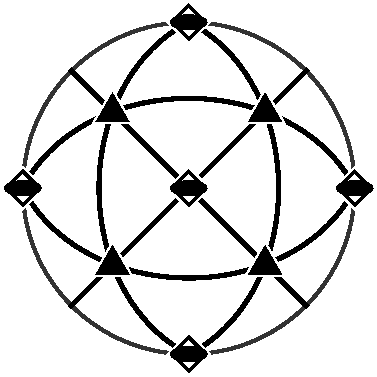
\includegraphics[width=\textwidth]{pic/43m}
      \subcaption{$\bar 43m$}
    \end{subfigure}
    \begin{subfigure}{0.3\textwidth}
      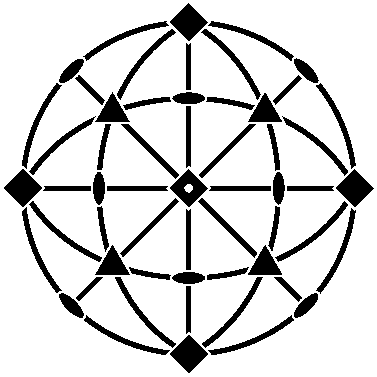
\includegraphics[width=\textwidth]{pic/m-3m}
      \subcaption{$m\bar 3 m$}
    \end{subfigure}

    \begin{subfigure}{0.3\textwidth}
      \centering
      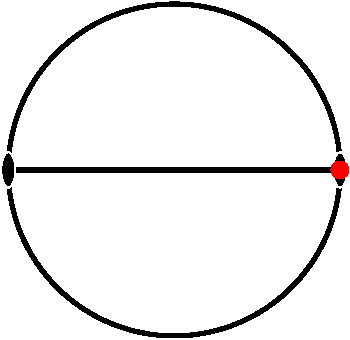
\includegraphics[width=0.95\textwidth]{pic/2mm}
      \caption{$2mm$}
    \end{subfigure}
    \begin{subfigure}{0.3\textwidth}
      \centering
      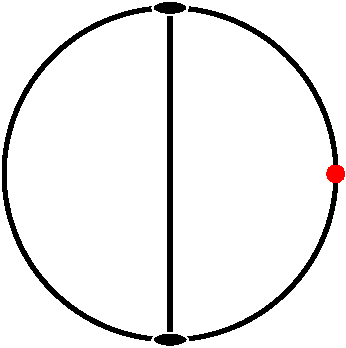
\includegraphics[width=0.95\textwidth]{pic/m2m}
      \caption{$m2m$}
    \end{subfigure}
    \begin{subfigure}{0.3\textwidth}
      \centering
      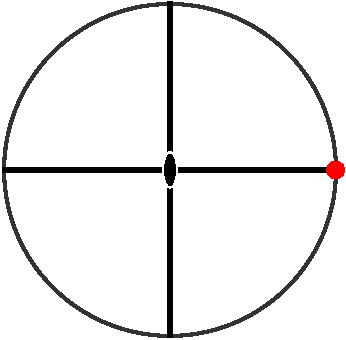
\includegraphics[width=0.95\textwidth]{pic/mm2}
      \caption{$mm2$}
    \end{subfigure}
  \end{figure}

\end{frame}

\subsection*{trigonal}

\begin{frame}

  \begin{figure}[H]
    \centering
    \begin{subfigure}{0.3\textwidth}
      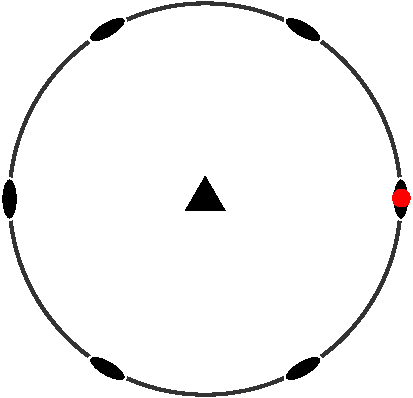
\includegraphics[width=\textwidth]{pic/sym321}
      \subcaption{$321$}
    \end{subfigure}
    \begin{subfigure}{0.3\textwidth}
      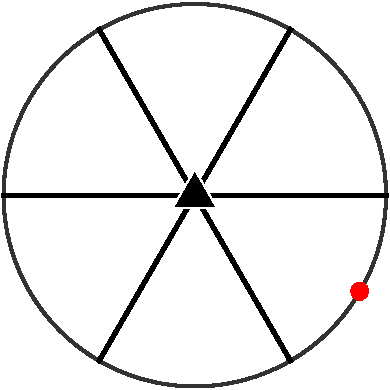
\includegraphics[width=\textwidth]{pic/sym3m1}
      \subcaption{$3m1$}
    \end{subfigure}
    \begin{subfigure}{0.3\textwidth}
      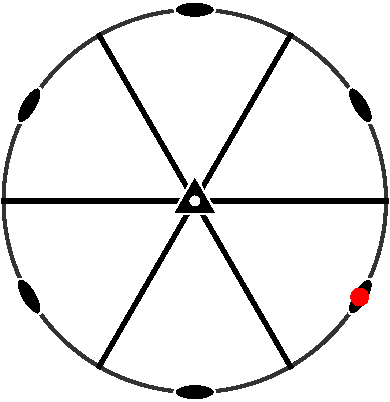
\includegraphics[width=\textwidth]{pic/sym-3m1}
      \caption{$\bar 3m1$}
    \end{subfigure}
    \begin{subfigure}{0.3\textwidth}
      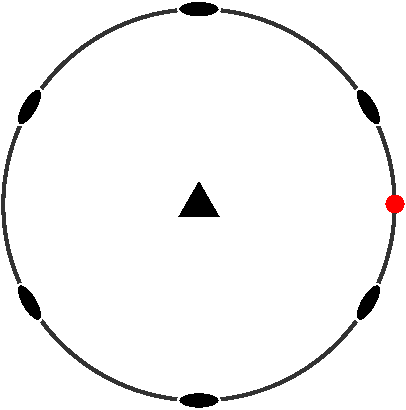
\includegraphics[width=\textwidth]{pic/sym312}
      \caption{$312$}
    \end{subfigure}
    \begin{subfigure}{0.3\textwidth}
      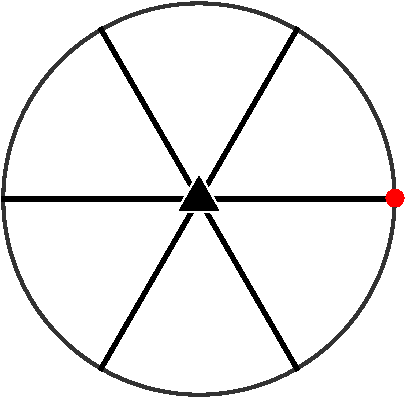
\includegraphics[width=\textwidth]{pic/sym31m}
      \caption{$31m$}
    \end{subfigure}
    \begin{subfigure}{0.3\textwidth}
      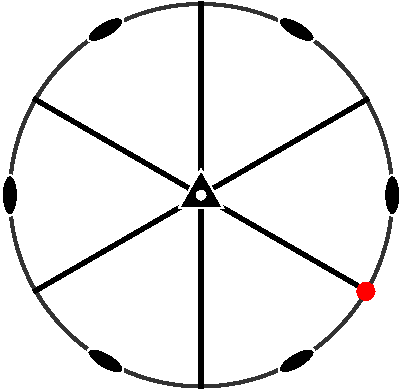
\includegraphics[width=\textwidth]{pic/sym-31m}
      \caption{$\bar 31m$}
    \end{subfigure}
  \end{figure}

\end{frame}


\subsection*{Crystal Symmetries}
\label{sec:crystal-symmetries}

\begin{frame}[fragile]
  \frametitle{Unit Cell, Reciprocal and Orthogonal Coordinate System}

  \begin{overlayarea}{\textwidth}{8cm}
    The unit cell of a crystal is specified by the length of its three edges
    $\vec a, \vec b, \vec c$ and by angles $\alpha, \beta, \gamma$ they enclose.

  \begin{lstlisting}[style=input]
C = crystalSymmetry('1',[a b c],[alpha beta gamma])
  \end{lstlisting}

  \begin{columns}
    \begin{column}{7.5cm}

      \begin{uncoverenv}<2->
        The axes of the reciprocal lattice are defined
        orthogonal to $\vec a, \vec b, \vec c$, i.e.
\vspace{-0.2cm}
\begin{equation*}
  \vec a^{*} = \frac{\vec b \times \vec c}{V}, \;
  \vec b^{*} = \frac{\vec c \times \vec a}{V}, \;
  \vec c^{*} = \frac{\vec a \times \vec b}{V}
\end{equation*}

\vspace{-0.4cm}

with  $V = \vec a \cdot (\vec b \times \vec c)$  volume of the unit cell
      \end{uncoverenv}

      \medskip

      \begin{uncoverenv}<3->
        We will need also an orthogonal coordinate system $(\vec x, \vec y,
        \vec z)$ fixed to the crystal.
      \end{uncoverenv}

      \medskip

      \begin{uncoverenv}<4->
        \alert{There are different conventions.}
      \end{uncoverenv}

  \end{column}

    \begin{column}{4.5cm}
      \begin{tikzpicture}[x  = {(-0.5cm,-0.5cm)},
        y  = {(0.9659cm,-0.25882cm)},
        z  = {(0cm,1cm)},
        scale = 2]

\draw[draw=green, dashed] (0,0,0) -- (1.2,0,0) -- (1,1,0) -- (-0.2,1,0) --
(0,1.2,1) -- (0.2,0.2,1) --  (1.4,0.2,1) -- (1.2,0,0);

\draw[draw=green, dashed] (0,1.2,1) -- (1.2,1.2,1) -- (1,1,0);
\draw[draw=green, dashed] (1.2,1.2,1) -- (1.4,0.2,1);


\draw[draw=green,very thick] (0,0,0) -- (1.2,0,0) node [anchor=north,color=green!70!black] {$\vec a$};
\draw[draw=green,very thick] (0,0,0) -- (-0.2,1,0) node [anchor=west,color=green!70!black] {$\vec b$};
\draw[draw=green,very thick] (0,0,0) -- (0.2,0.2,1) node[anchor=south,color=green!70!black] {$\vec c$};

\only<1>{
\draw[draw=green] (0.3,0,0) arc (250:329:0.3cm);% node {$\alpha$};
\draw[draw=green] (-0.03,0.2,0) arc (0:68:0.3cm);% node {$\alpha$};
\draw[draw=green] (0.3,0,0) arc (200:112:0.3cm);% node {$\alpha$};
\node at (0.15,0.01,0.1)[color=green!70!black]{$\beta$};
\node at (0.01,0.15,0.1)[color=green!70!black]{$\alpha$};
\node at (0.15,0.1,0)[color=green!70!black]{$\gamma$};
}


\only<2->{
\draw[->,draw=red,very thick] (0,0,0) -- (0,0,1.2) node [anchor=west,color=red!70!black] {$\vec c^{*}$};
\draw[->,draw=red,very thick] (0,0,0) -- (1,0.2,-0.24) node [anchor=west,color=red!70!black] {$\vec a^{*}$};
\draw[->,draw=red,very thick] (0,0,0) -- (0,1.2,-0.24) node [anchor=north,color=red!70!black] {$\vec b^{*}$};
}

\only<3|handout>{
\draw[->,draw=black,ultra thick] (0,0,0) -- (1,0,0) node
[anchor=north,color=black] {$\vec{\mathbf x}$};
\draw[->,draw=black,ultra thick] (0,0,0) -- (0,1,0) node
[anchor=north,color=black] {$\vec{\mathbf y}$};
\draw[->,draw=black,ultra thick] (0,0,0) -- (0,0,1) node
[anchor=east,color=black] {$\vec{\mathbf z}$};
}

\only<4>{
\draw[->,draw=black,ultra thick] (0,0,0) -- (1,0.2,0) node
[anchor=north,color=black] {$\vec{\mathbf x}$};
\draw[->,draw=black,ultra thick] (0,0,0) -- (-0.2,1,0) node
[anchor=north,color=black] {$\vec{\mathbf y}$};
\draw[->,draw=black,ultra thick] (0,0,0) -- (0,0,1) node
[anchor=east,color=black] {$\vec{\mathbf z}$};
}

\end{tikzpicture}

\end{column}
\end{columns}

\begin{onlyenv}<3|handout>
  \begin{lstlisting}[style=input]
CS = crystalSymmetry('321',[a b c],'X||a','Z||c*')
  \end{lstlisting}
\end{onlyenv}

\begin{onlyenv}<4->
  \begin{lstlisting}[style=input]
CS = crystalSymmetry('321',[a b c],'X||b','Z||c*')
\end{lstlisting}
\alert{The alignment of $\vec x$, $\vec y$, $\vec z$ is important as the Euler angles
refer to them.}
\end{onlyenv}

\end{overlayarea}

\end{frame}

\section{Miller Indices}
\label{sec:miller-indices}

\subsection*{definition}
\label{sec:definition}

\begin{frame}[fragile]
  \frametitle{Miller Indices - Crystal Fixed Directions}

  A direction with respect to the crystal coordinate system  $\mathbf C$

  \begin{columns}
    \begin{column}{7cm}

      \begin{overlayarea}{8cm}{8cm}

        \begin{equation*}
          \vec m = u \cdot \vec a+ v \cdot \vec b + w \cdot \vec c.
        \end{equation*}

    \begin{onlyenv}<2->
\begin{lstlisting}[style=input]
CS = crystalSymmetry('mmm',[1 2 3])
m  = Miller(-1,1,1,CS,'uvw')
\end{lstlisting}
\end{onlyenv}
\begin{onlyenv}<2>
\vspace{-.3cm}\begin{lstlisting}[style=output]
m = /+Miller+/ (show methods, plot)
  size: 1 x 1
  symmetry: mmm
  u -1
  v 1
  w 1
\end{lstlisting}
\end{onlyenv}

    \begin{onlyenv}<3->
A direction in reciprocal coordinates
\begin{equation*}
  \vec n = h \cdot \vec a^{*}+ k \cdot \vec b^{*} + \ell \cdot \vec c^{*}.
\end{equation*}
\begin{lstlisting}[style=input]
n  = Miller(-1,1,1,CS,'hkl')
\end{lstlisting}
\end{onlyenv}
\begin{onlyenv}<3>
  \vspace{-.3cm}
  \begin{lstlisting}[style=output]
n = /+Miller+/ (show methods, plot)
  size: 1 x 1
  symmetry: mmm
  h -1
  k 1
  l 1
\end{lstlisting}
\end{onlyenv}

\medskip

\begin{onlyenv}<4->
  A direction in the orthogonal coordinate system
  \begin{lstlisting}[style=input]
m = Miller(vector3d.X,CS)
\end{lstlisting}
\end{onlyenv}
\end{overlayarea}
\end{column}
    \begin{column}{4cm}

      \begin{overlayarea}{4cm}{7cm}

      \begin{center}
        \includegraphics<2>[width=4cm]{pic/MillerUVW}
%        \includegraphics<3>[width=4cm]{pic/MillerHKL}
        \includegraphics<3->[width=4cm]{pic/MillerPlane}
      \end{center}
      \vspace{-0.2cm}
        \begin{onlyenv}<2-|handout>
          \begin{lstlisting}[style=input]
plot(m,'labeled')
          \end{lstlisting}%
        \end{onlyenv}%
        \vspace{-0.25cm}
        \begin{onlyenv}<3->%
          \begin{lstlisting}[style=input]
hold all
plot(n,'labeled')
          \end{lstlisting}%
        \end{onlyenv}%
        \vspace{-0.25cm}
        \begin{onlyenv}<3->%
          \begin{lstlisting}[style=input]
plot(n,'plane')
          \end{lstlisting}
        \end{onlyenv}
          \end{overlayarea}
      \end{column}
    \end{columns}

\end{frame}

\subsection*{The trigonal case}

\begin{frame}[fragile]
  \frametitle{Trigonal and Hexagonal Symmetries}

  \vspace{-.3cm}

  \begin{center}
    \begin{minipage}[t]{0.3\linewidth}
       \vspace{0pt}
      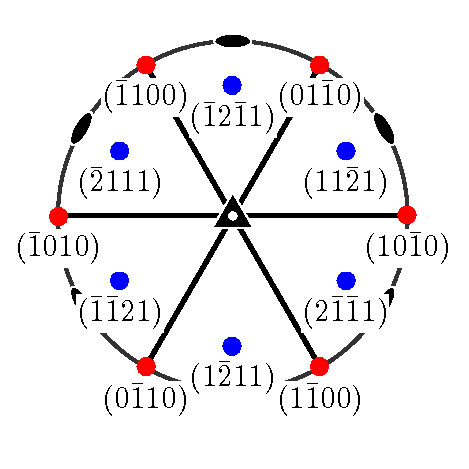
\includegraphics[width=\textwidth]{pic/hkl}
    \end{minipage}
    \hfill
    \begin{minipage}[t]{0.3\linewidth}
       \vspace{0pt}
      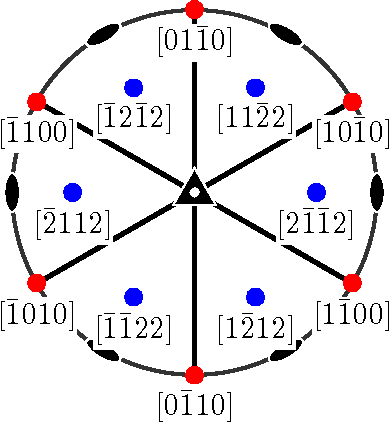
\includegraphics[width=\textwidth]{pic/uvtw}
    \end{minipage}
    \hfill
    \begin{minipage}[t]{0.34\linewidth}
       \vspace{0pt}
      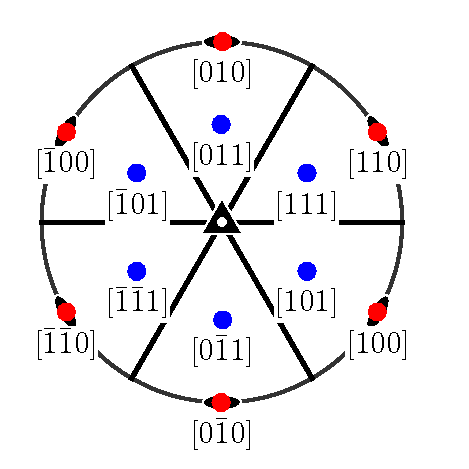
\includegraphics[width=\textwidth]{pic/uvw}
    \end{minipage}
  \end{center}

  define lists of crystal directions
  \vspace{-.2cm}
  \begin{lstlisting}[style=input]
m = Miller({1 0 -1 0},{1 1 -2 1},CS,'hkil')
m = Miller({1 0 -1 0},{1 1 -2 2},CS,'UVTW')
m = Miller({1 0 0},{1 0 1},CS,'uvw')
  \end{lstlisting}%

  \medskip

  Plot all symmetrically equivalent directions
    \vspace{-.2cm}
  \begin{lstlisting}[style=input]
plot(m,'symmetrised','labeled')
  \end{lstlisting}



\end{frame}

\subsection*{Calculations}

\begin{frame}[fragile]
  \frametitle{Calculating with Crystal Directions}

   \begin{columns}
     \begin{column}{8.6cm}
         \begin{overlayarea}{\textwidth}{8cm}
           Find all symmetrically equivalent directions
           \vspace{-0.1cm}
           \begin{lstlisting}[style=input]
CS = loadCIF('quartz')
m = Miller(1,1,-2,1,CS,'hkil')
symmetrise(m)
           \end{lstlisting}

           \begin{onlyenv}<1>
             \vspace{-.3cm}
            \begin{lstlisting}[style=output]
ans = /+Miller+/ (show methods, plot)
  size: 6 x 1
  mineral: Quartz (P 32 2 1, X||a*, Y||b, Z||c*)
  h  1 -2  1  1 -2  1
  k  1  1 -2 -2  1  1
  i -2  1  1  1  1 -2
  l  1  1  1 -1 -1 -1
       \end{lstlisting}
     \end{onlyenv}

        \pause
        \medskip

        Change from reciprocal coordinate system to $\vec a$, $\vec b$,
        $\vec c$
        \vspace{-0.1cm}
  \begin{lstlisting}[style=input]
m.dispStyle = 'UVTW'
  \end{lstlisting}
           \begin{onlyenv}<2>
             \vspace{-.3cm}
             \begin{lstlisting}[style=output]
m = /+Miller+/ (show methods, plot)
  size: 6 x 1
  mineral: Quartz (P 32 2 1, X||a*, Y||b, Z||c*)
  U  0.0828
  V  0.0828
  T -0.1655
  W  0.1027
       \end{lstlisting}
     \end{onlyenv}

        \pause
        \vspace{-.3cm}

  \begin{lstlisting}[style=input]
round(m)
  \end{lstlisting}
           \begin{onlyenv}<3>
             \vspace{-.3cm}
             \begin{lstlisting}[style=output]
ans = /+Miller+/ (show methods, plot)
  size: 6 x 1
  mineral: Quartz (P 32 2 1, X||a*, Y||b, Z||c*)
  U  4
  V  4
  T -8
  W  5
       \end{lstlisting}
     \end{onlyenv}

        \pause
        \medskip

        Access the coordinates and properties
        \vspace{-0.1cm}
  \begin{lstlisting}[style=input]
m.U, m.hkl, m.uvw, m.UVTW
m.dspacing % d-spacing of planes
  \end{lstlisting}

        \pause
        \medskip

        angle modulo symmetry
        \vspace{-0.1cm}
        \begin{lstlisting}[style=input]
angle(m1,m2) / degree
\end{lstlisting}


 \end{overlayarea}

     \end{column}
     \begin{column}{3.5cm}
       \includegraphics<1->[width=3.5cm]{pic/MillerSymmetrised}%\\
%       \includegraphics<1->[width=4cm]{pic/Symmetry}
     \end{column}
   \end{columns}
\end{frame}

\section{Orientations}
\label{sec:orientations}

\subsection*{Definition}

\begin{frame}
  \frametitle{Crystal Orientations}

  \begin{columns}

    \begin{column}{6.3cm}

      \begin{overlayarea}{6.4cm}{8cm}
        Let a vector $\vec v$ be given by specimen coordinates
        $(r_{1},r_{2},r_{3})^{t}$ \underline{and} crystal coordinates
        $(h_{1},h_{2},h_{3})^{t}$, i.e.,
        \begin{equation*}
          \vec v = r_{1} \vec X + r_{2} \vec Y + r_{3} \vec Y
                 = h_{1} \vec x + h_{2} \vec y + h_{3} \vec z.
        \end{equation*}

        \pause

        The coordinate transform $\mathbf O$ with
      \begin{equation*}
        \left(r_{1},r_{2},r_{3}\right)^{t}
        =
         \mathbf O
         \left(
          h_{1},h_{2},h_{3} \right)^{t}
      \end{equation*}
      is called \alert{crystal orientation}.

      \pause
      \medskip

      The orientation $\mathbf O$ maps the specimen coordinate system $\vec X,
      \vec Y, \vec Z$ onto the crystal coordinate systems $\vec x, \vec y,
      \vec z$.

      \pause
      \medskip

      The orientation $\mathbf O$ is well defined only up the crystal
      symmetry.

    \end{overlayarea}
  \end{column}

    \begin{column}{5cm}

      \onslide<1->
      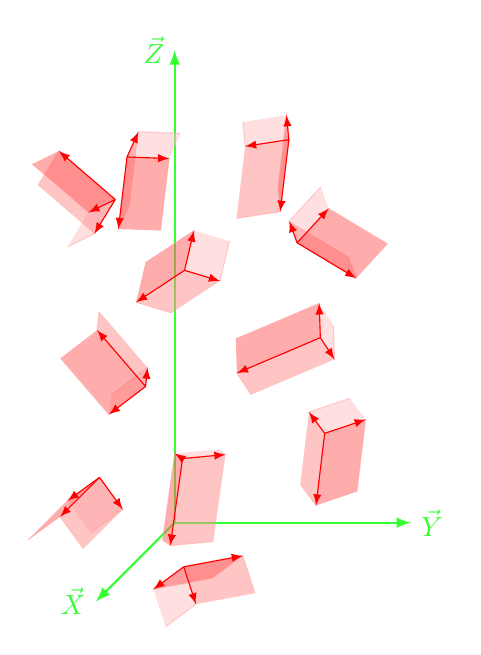
\begin{tikzpicture}[scale=0.5]

        \draw[->, >=latex, color=green!80, thick] (0,0) -- (0,12) node[left] {$\vec Z$};
        \draw[->, >=latex, color=green!80, thick] (0,0) -- (6,0) node[right] {$\vec Y$};
        \draw[->, >=latex, color=green!80, thick] (0,0) -- (-2,-2) node[left] {$\vec X$};
%        \draw (6,11) node[color=green]{$K_S$};

        \foreach \xpos/\ypos/\xx/\xy/\yx/\yy/\zx/\zy
        in {
0.20/1.63/-0.20/0.13/1.09/0.10/-0.31/-2.21,
3.11/7.11/0.80/0.87/-0.20/0.55/1.50/-0.90,
3.70/4.70/-0.03/0.87/0.36/-0.55/-2.12/-0.90,
-1.91/1.15/-0.81/-0.59/0.59/-0.81/-1.00/-1.00,
2.90/9.73/-0.06/0.62/-1.11/-0.17/-0.22/-1.83,
%-0.67/6.44/-0.86/0.34/0.59/1.05/0.81/-0.37,
%1.13/9.19/-0.79/-0.78/0.37/-0.79/-1.40/0.21,
%2.28/0.74/0.44/1.02/-0.70/0.43/1.50/0.28,
%0.70/0.07/-0.06/1.08/-0.83/-0.25/1.50/0.28,
3.81/2.27/1.04/0.35/-0.40/0.54/-0.22/-1.83,
%-1.71/7.06/-0.16/0.06/0.61/1.04/1.85/-0.81,
%3.37/1.43/-0.61/-0.60/0.93/-0.23/-0.22/-1.83,
%-0.49/9.19/0.24/0.73/0.27/0.84/-2.12/0.28,
-1.21/9.29/1.07/-0.04/0.29/0.64/-0.22/-1.83,
%2.21/8.17/1.01/0.53/0.27/0.34/0.81/-1.85,
-0.74/3.46/-0.93/-0.71/0.05/0.48/-1.23/1.43,
-1.51/8.21/-0.68/-0.33/-0.53/-0.87/-1.43/1.23,
%1.37/1.83/1.07/0.51/-0.29/0.99/-0.22/0.21,
0.25/6.41/0.24/1.01/0.90/-0.27/-1.23/-0.81,
0.23/-1.12/-0.77/-0.57/0.31/-0.95/1.50/0.28
        }
        \fillcrystal{\xpos,\ypos}{\xx,\xy}{\yx,\yy}{\zx,\zy}{color=red};

      \end{tikzpicture}
    \end{column}
\end{columns}
\end{frame}

\subsection*{Defining Orientations}
\label{sec:defin-orient}

\begin{frame}[fragile]
  \frametitle{Defining Orientations}

    \begin{overlayarea}{\textwidth}{8cm}
      define an orientation by Euler angles
  \begin{lstlisting}[style=input]
CS = crystalSymmetry('321')
SS = specimenSymmetry('1')
O  = orientation('Euler',10*degree,5*degree,0,CS,SS)
  \end{lstlisting}
  \begin{onlyenv}<1>
    \vspace{-.3cm}
  \begin{lstlisting}[style=output]
O = /+orientation+/ (show methods, plot)
  size: 1 x 1
  crystal symmetry: 321, X||a*, Y||b, Z||c*
  sample symmetry : 1

  Bunge Euler angles in degree
  Psi Theta   Phi Inv.
   10     5     0    0
  \end{lstlisting}
  \end{onlyenv}

  \pause
  import orientations
  \begin{lstlisting}[style=input]
O  = loadOrientation('filename',CS,SS,...
'ColumnNames',{'phi1','Phi','phi2'})
  \end{lstlisting}
  \begin{onlyenv}<2>
    \vspace{-.3cm}
  \begin{lstlisting}[style=output]
O = /+orientation+/ (show methods, plot)
  size: 1000 x 1
  crystal symmetry: 321, X||a*, Y||b, Z||c*
  sample symmetry : 1
  \end{lstlisting}
  \end{onlyenv}

\pause

define orientations by Miller indices
   \begin{lstlisting}[style=input]
O  = orientation('Miller',[h k l],[u,v,w],CS,SS)
  \end{lstlisting}

\pause

standard orientations: \texttt{Cube, CubeND22, CubeND45, CubeRD, Goss,
invGoss, Copper, Copper2, SR, SR2, SR3, SR4, Brass, Brass2, PLage, PLage2,
QLage, QLage2, QLage3, QLage4}

\begin{lstlisting}[style=input]
O  = brassOrientation(CS,SS)
\end{lstlisting}
\end{overlayarea}
\end{frame}

\subsection*{Calculating with Orientations}
\label{sec:calc-with-orient}

\begin{frame}[fragile,fragile,fragile,fragile]
  \frametitle{Calculating with Orientations}


  \begin{overlayarea}{\textwidth}{8cm}
  find all symmetrically equivalent orientations
\begin{lstlisting}[style=input]
symmetrise(O)
\end{lstlisting}
  \begin{onlyenv}<1>
    \vspace{-.3cm}
    \begin{lstlisting}[style=output]
ans = /+orientation+/ (show methods, plot)
  size: 6 x 1
  crystal symmetry: 321, X||a*, Y||b, Z||c*
  sample symmetry : 1

  Roe Euler angles in degree
  Psi Theta   Phi Inv.
   10     5     0    0
   10     5   120    0
   10     5   240    0
  190   175    60    0
  190   175   180    0
  190   175   300    0
\end{lstlisting}
  \end{onlyenv}

  \pause
  \medskip

  convert crystal into specimen coordinates
\begin{lstlisting}[style=input]
h = Miller(1,0,-1,0,CS);
r = O * h
\end{lstlisting}
  \begin{onlyenv}<2>
    \vspace{-.3cm}
    \begin{lstlisting}[style=output]
r = /+vector3d+/ (show methods, plot)
  size: 1 x 1
         x        y        z
  0.984808 0.173648        0
\end{lstlisting}
  \end{onlyenv}

  \pause
  \medskip

  convert specimen into crystal coordinates
\begin{lstlisting}[style=input]
inv(O) * r
\end{lstlisting}
  \begin{onlyenv}<3>
    \vspace{-.3cm}
    \begin{lstlisting}[style=output]
ans = /+Miller+/ (show methods, plot)
  size: 1 x 1
  symmetry: 321, X||a*, Y||b, Z||c*
  h  1
  k  0
  i -1
  l  0
\end{lstlisting}
  \end{onlyenv}

  \pause
  \medskip

  change specimen coordinates
  \begin{lstlisting}[style=input]
R  = rotation('axis',vector3d.Z,'angle',90*degree)
O2 = R * O1
\end{lstlisting}
\end{overlayarea}

\end{frame}


\subsection*{Pole Figures}

\begin{frame}[fragile]
  \frametitle{Pole Figures and Inverse Pole Figures}

  \begin{columns}
    \begin{column}{8.5cm}
      Lattice planes in specimen coordinates
      \begin{lstlisting}[style=input]
h = Miller({1 0 0}, {0 1 0}, O.CS)
plot(symmetrise(O) * h(1))
plot(O * symmetrise(h(1)))
      \end{lstlisting}

      \pause
      \medskip

      \begin{lstlisting}[style=input]
plotPDF(O,h)
      \end{lstlisting}
      \pause
      \vspace{-0.3cm}
      \begin{lstlisting}[style=input]
plotPDF(O,h,'contourf')
      \end{lstlisting}

      \pause
      \medskip

      specimen directions in crystal coordinates
      \begin{lstlisting}[style=input]
plot(symmetrise(inv(O)) * vector3d.X)
plot(symmetrise(inv(O) * vector3d.X))
      \end{lstlisting}
      \pause
      \vspace{-0.3cm}
      \begin{lstlisting}[style=input]
v = [vector3d.X, vector3d.Y]
plotIPDF(O,v)
      \end{lstlisting}
      \pause
      \vspace{-0.3cm}
      \begin{lstlisting}[style=input]
plotIPDF(O,v,'contourf')
      \end{lstlisting}


    \end{column}
    \begin{column}{3.5cm}

      \begin{onlyenv}<1>
        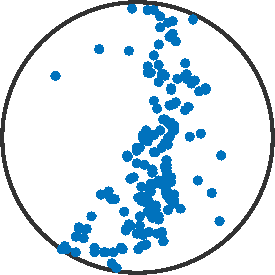
\includegraphics[width=\textwidth]{pic/pfSimple}
      \end{onlyenv}

      \begin{onlyenv}<2>
        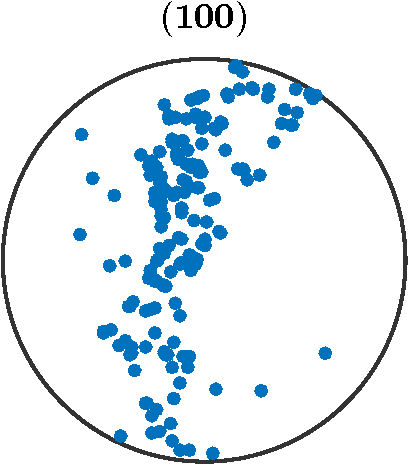
\includegraphics[width=0.95\textwidth]{pic/pfSimple100}

        \medskip

        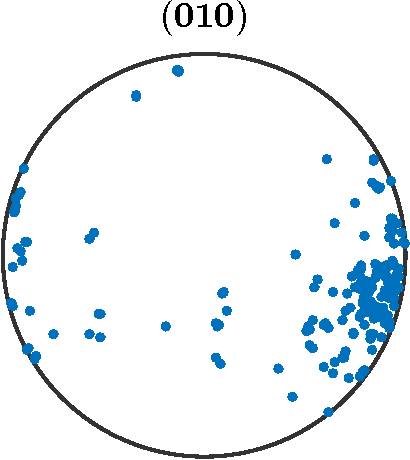
\includegraphics[width=0.95\textwidth]{pic/pfSimple010}
      \end{onlyenv}

      \begin{onlyenv}<3>
        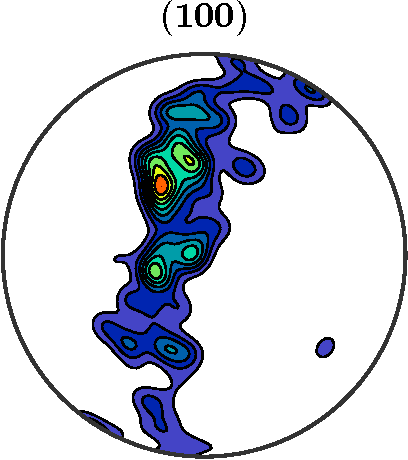
\includegraphics[width=0.95\textwidth]{pic/pfSimple100Smooth}

        \medskip

        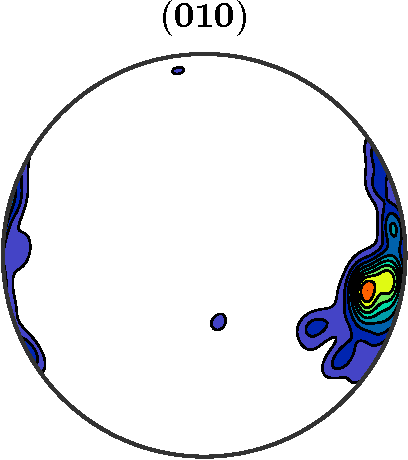
\includegraphics[width=0.95\textwidth]{pic/pfSimple010Smooth}
      \end{onlyenv}

      \begin{onlyenv}<4>
        
\includegraphics[width=\textwidth]{pic/ipfSimple}
      \end{onlyenv}

      \begin{onlyenv}<5>
        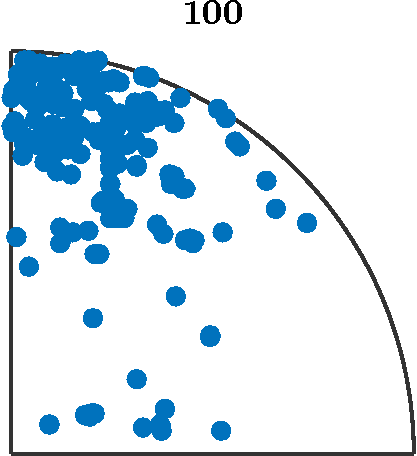
\includegraphics[width=0.95\textwidth]{pic/ipfSimple100}

        \medskip

        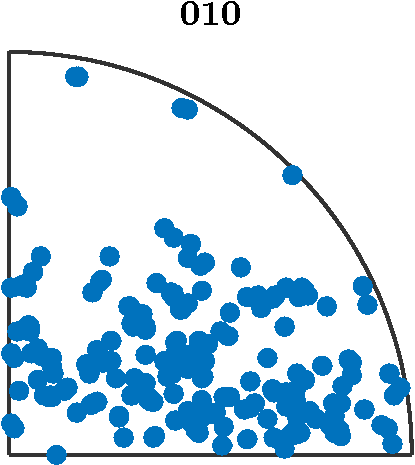
\includegraphics[width=0.95\textwidth]{pic/ipfSimple010}
      \end{onlyenv}

      \begin{onlyenv}<6>
        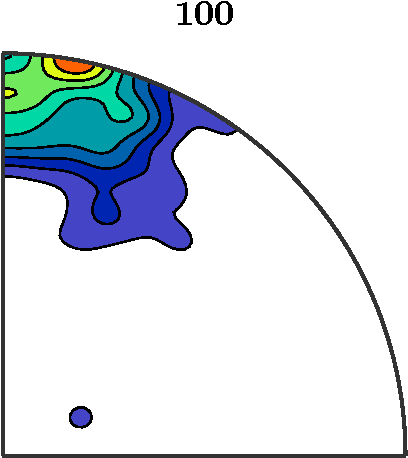
\includegraphics[width=0.95\textwidth]{pic/ipfSimple100Smooth}

        \medskip

        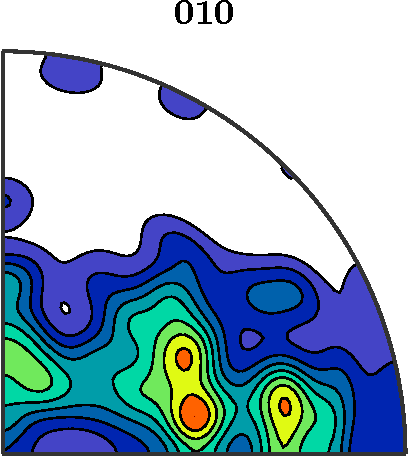
\includegraphics[width=0.95\textwidth]{pic/ipfSimple010Smooth}
      \end{onlyenv}
    \end{column}
  \end{columns}

\end{frame}

\subsection*{ODF Plots}

\begin{frame}[fragile]
  \frametitle{Plotting in Orientation Space}

  \begin{onlyenv}<1>
    \begin{lstlisting}[style=input]
plotSection(O,'phi2',(0:30:150)*degree)
    \end{lstlisting}
    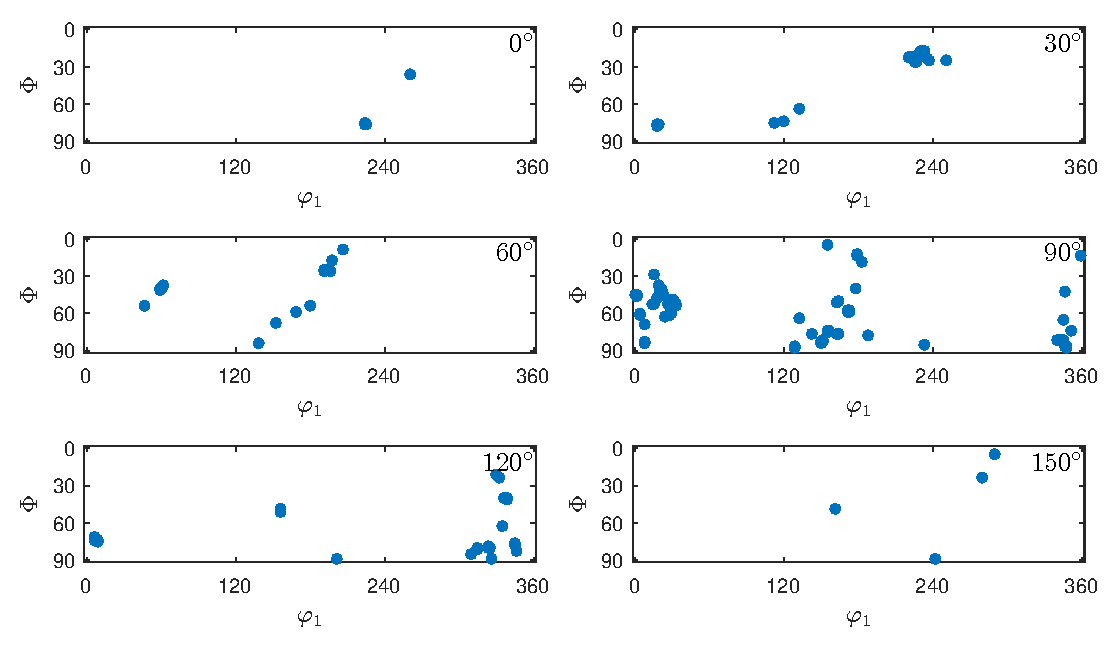
\includegraphics[width=\textwidth]{pic/odfOri}
  \end{onlyenv}

  \begin{onlyenv}<2>
    \begin{lstlisting}[style=input]
plotSection(O,'phi2',(0:30:150)*degree,...
            'contourf','halfwidth',10*degree)
    \end{lstlisting}
    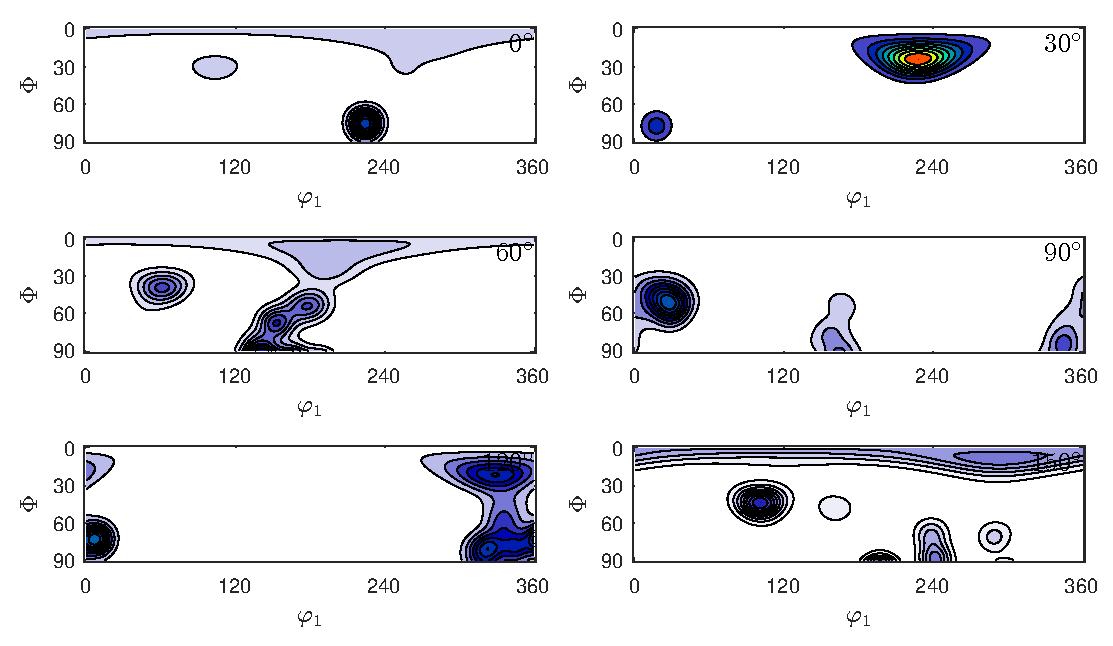
\includegraphics[width=0.95\textwidth]{pic/odfOriSmooth}
  \end{onlyenv}

    \begin{onlyenv}<3>
    \begin{lstlisting}[style=input]
plotSection(O,'sigma',(0:30:150)*degree,'contourf')
    \end{lstlisting}
    \vspace{-0.3cm}
    \begin{center}
      \includegraphics[width=0.9\textwidth]{pic/odfOriSmoothSigma}
    \end{center}
  \end{onlyenv}

  \begin{onlyenv}<4>
    \begin{lstlisting}[style=input]
plotSection(O,'AxisAngle',(10:15:115)*degree,...
            'contourf')
    \end{lstlisting}
    \vspace{-0.3cm}
    \begin{center}
      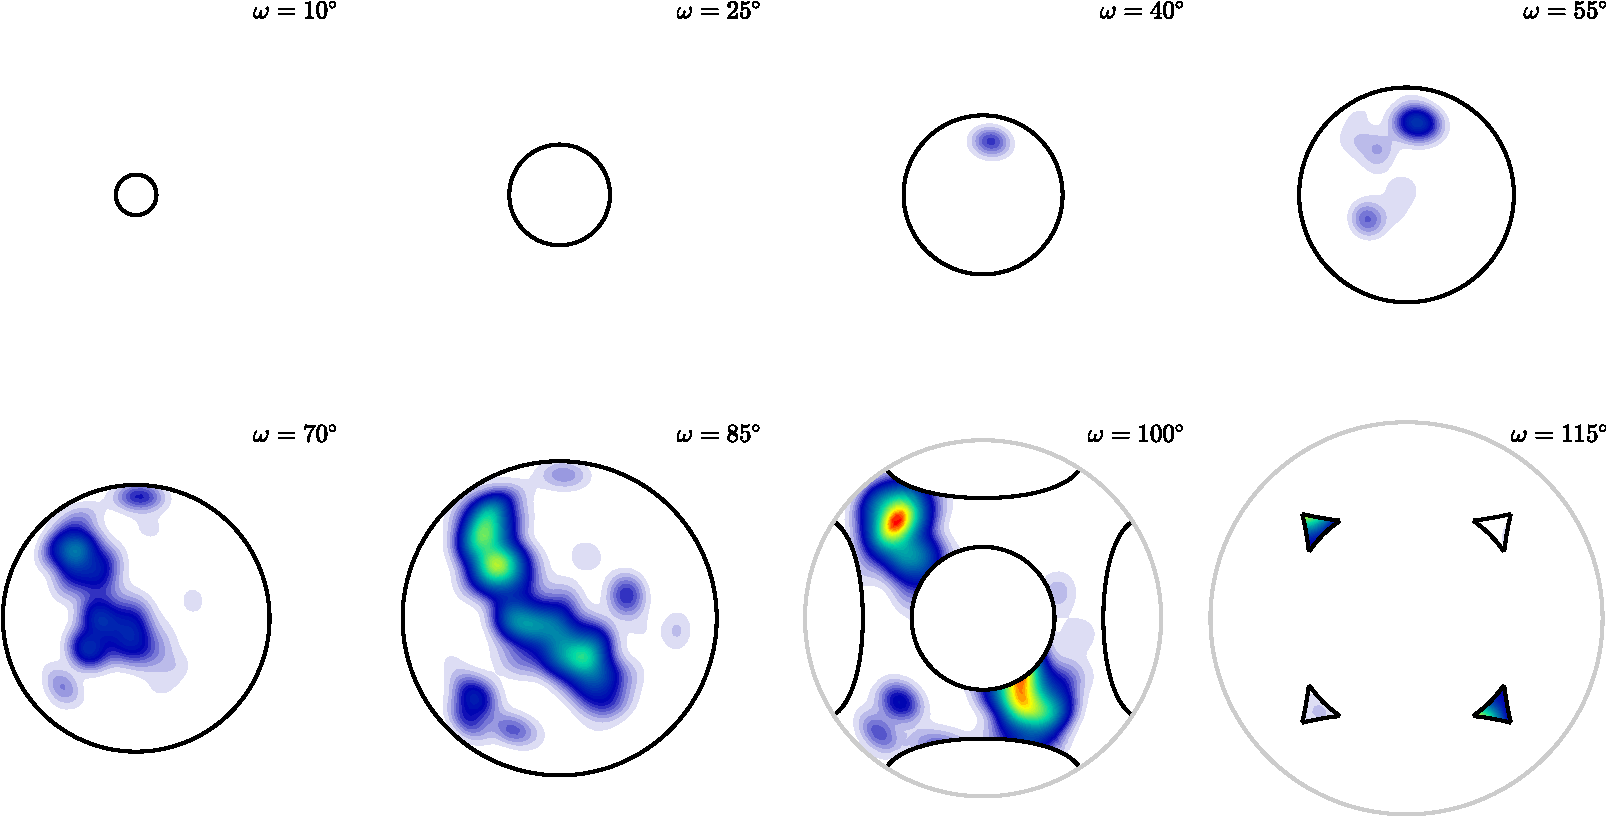
\includegraphics[width=\textwidth]{pic/odfOriSmoothAxisAngle}
    \end{center}
  \end{onlyenv}

\end{frame}

\subsection*{The Orientation Space}

\begin{frame}[fragile]
  \frametitle{The Orientation Space}

  \begin{columns}
    \begin{column}{0.55\textwidth}

      \begin{lstlisting}[style=input]
plot(orientationRegion)
      \end{lstlisting}

      \pause

      \vspace{-0.1cm}
      \begin{lstlisting}[style=input]
cs = crystalSymmetry('mmm')
oR = cs.fundamentalRegion
plot(oR,'color','r')
\end{lstlisting}

\pause

\vspace{-0.1cm}
      \begin{lstlisting}[style=input]
cs = crystalSymmetry('321')
oR = cs.fundamentalRegion
plot(oR,'color','r')
\end{lstlisting}

\pause

\vspace{-0.1cm}
      \begin{lstlisting}[style=input]
cs = crystalSymmetry('432')
oR = cs.fundamentalRegion
plot(oR,'color','r')
      \end{lstlisting}

    \end{column}
    \begin{column}{0.45\textwidth}
      \only<1>{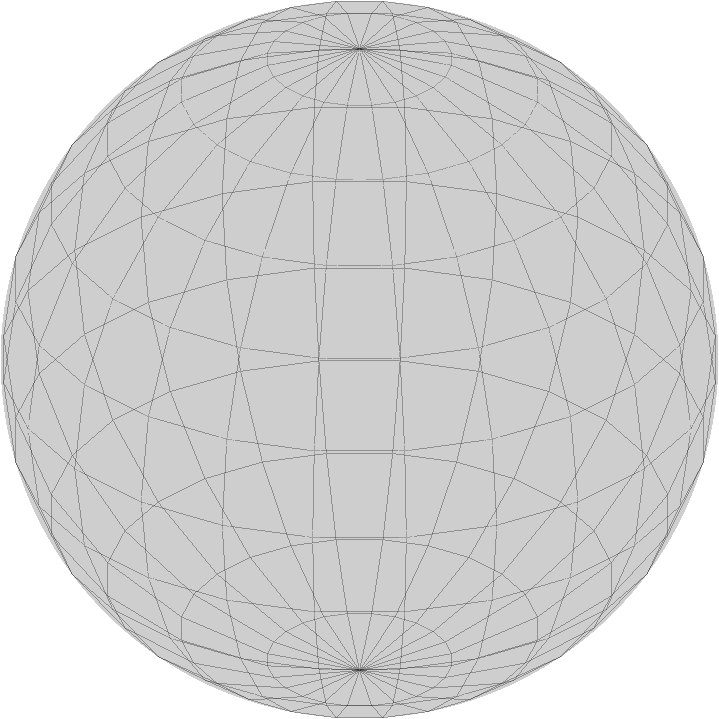
\includegraphics[width=\textwidth]{pic/oR1}}
      \only<2>{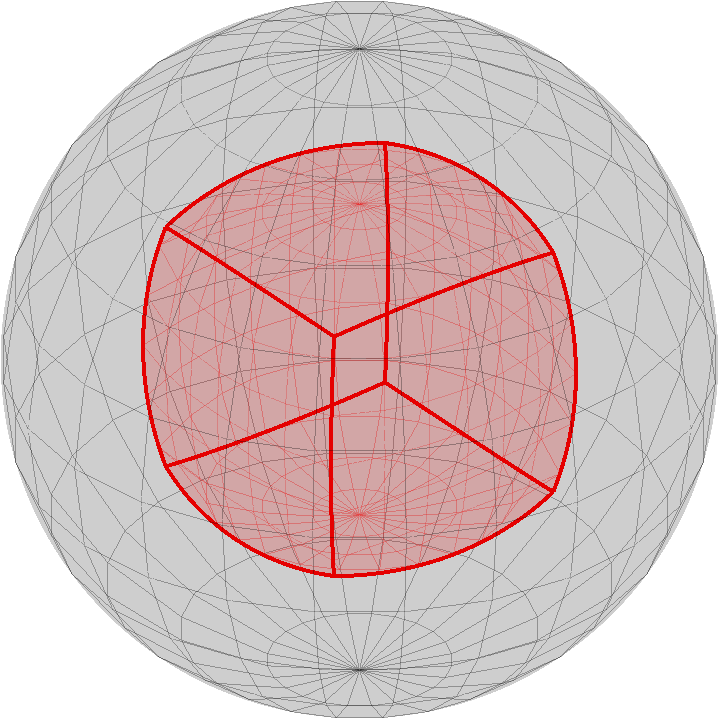
\includegraphics[width=\textwidth]{pic/oRmmm}}
      \only<3>{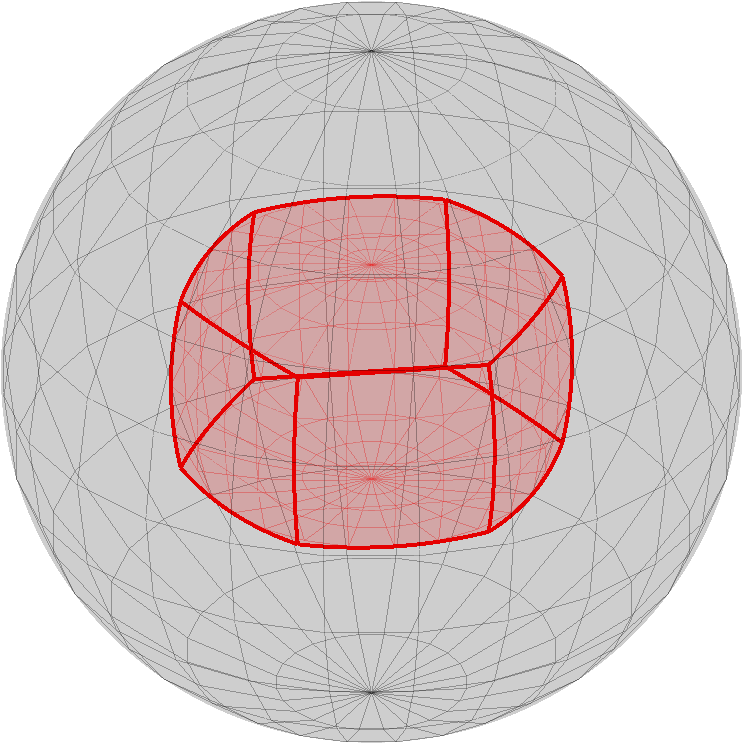
\includegraphics[width=\textwidth]{pic/oR321}}
      \only<4->{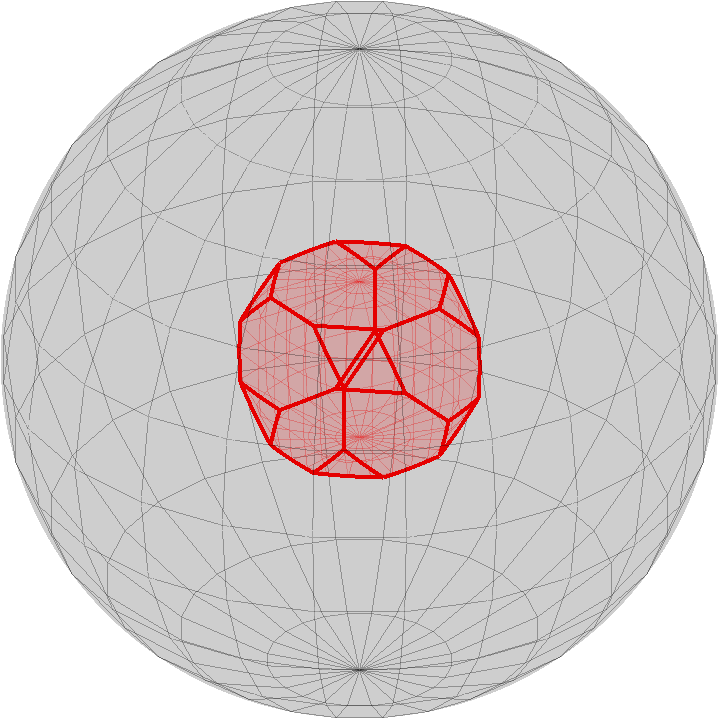
\includegraphics[width=\textwidth]{pic/oR432}}
    \end{column}
  \end{columns}

  \pause

  \begin{lstlisting}[style=input]
oR.V, oR.N, oR.checkInside, oR.axisSector(omega),
oR.maxAngle(axes), oR.minAngle,
oR.calcAxisDistribution, oR.calcAngleDistribution
  \end{lstlisting}


\end{frame}

\subsection*{Operations on Orientations}

\begin{frame}[fragile]
  \frametitle{Operations on Orientations}

%   the misorientation angle and axis
%   \begin{lstlisting}[style=input]
% angle(ori1,ori2) / degree
% axis(ori1,ori2)
%   \end{lstlisting}

%   \begin{onlyenv}<1>
%     \begin{lstlisting}[style=output]
% ans = /+Miller+/ (show methods, plot)
%   size: 1 x 1
%   mineral: Forsterite (mmm)
%   h 2.729
%   k 7.6909
%   l 1.9193
%     \end{lstlisting}
%   \end{onlyenv}

%   \pause
%   \medskip

mean orientation
  \begin{lstlisting}[style=input]
mean(O)
  \end{lstlisting}

  \begin{onlyenv}<1>
    \begin{lstlisting}[style=output]
ans = /+orientation+/ (show methods, plot)
  size: 1 x 1
  crystal symmetry : Forsterite (mmm)
  specimen symmetry: 1

  Bunge Euler angles in degree
     phi1     Phi    phi2    Inv.
  342.532 68.3179 284.955       0
    \end{lstlisting}
  \end{onlyenv}

\pause
\medskip

  mean orientation spread
  \begin{lstlisting}[style=input]
mean(angle(O,mean(O)))./degree
  \end{lstlisting}

  \begin{onlyenv}<2>
    \begin{lstlisting}[style=output]
ans =

   47.2287
\end{lstlisting}
  \end{onlyenv}

\pause
\medskip

volume portions
\begin{lstlisting}[style=input]
volume(O,mean(O),10*degree)
fibreVolume(O,Miller(1,0,0,O.CS),vector3d.X,5*degree)
\end{lstlisting}

\pause
\medskip

export to ASCII file
\begin{lstlisting}[style=input]
export(O,'file.txt','bunge','degree')
\end{lstlisting}

\end{frame}


\end{document}

\section{Misorientations}


\subsection*{Coordinate Transforms}
\label{sec:orientations}


\begin{frame}[fragile]
  \frametitle{Coordinate Transforms}

  \begin{overlayarea}{\textwidth}{8cm}
  Remember, an orientation converts crystal into specimen
  coordinates
  \vspace{-.2cm}
  \begin{lstlisting}[style=input]
O1 = orientation('Euler',0,0,0,CS_Mag)
r = O1 * Miller(1,1,1,CS_Mag)
\end{lstlisting}
  \begin{onlyenv}<1>
\vspace{-.3cm}\begin{lstlisting}[style=output]
r = /+vector3d+/ (show methods, plot)
 size: 1 x 1
         x        y        z
  0.119107 0.119107 0.119107
\end{lstlisting}
  \end{onlyenv}

  \pause
  \medskip

  The inverse of an orientation converts specimen into crystal coordinates
  \vspace{-.2cm}
  \begin{lstlisting}[style=input]
O2 = orientation('Euler',...
       135*degree,55*degree,60*degree,CS_Hem)
inv(O2) * r
\end{lstlisting}
  \begin{onlyenv}<2>
    \vspace{-.3cm}
    \begin{lstlisting}[style=output]
ans = /+Miller+/ (show methods, plot)
 size: 1 x 1
 mineral: Hematite (-3m1, X||a*, Y||b, Z||c)
  h 0
  k 0
  i 0
  l 1

\end{lstlisting}
  \end{onlyenv}

  \pause
  \medskip

  Hence, $\text{\bf inv}(\mathbf{O2}) \cdot \mathbf{O1}$ converts crystal  into
  crystal coordinates
    \vspace{-.2cm}
  \begin{lstlisting}[style=input]
O2 = inv(O2) * O1 * Miller(1,1,1,0,CS_Mag)
  \end{lstlisting}
  \begin{onlyenv}<3>
    \vspace{-.3cm}
    \begin{lstlisting}[style=output]
ans = /+Miller+/ (show methods, plot)
 size: 1 x 1
 mineral: Hematite (-3m1, X||a*, Y||b, Z||c)
  h 0
  k 0
  i 0
  l 1

\end{lstlisting}
  \end{onlyenv}

\end{overlayarea}

\end{frame}



\subsection*{Misorientations}
\label{sec:orientations2}

\begin{frame}[fragile]
  \frametitle{Misorientations}

  \begin{overlayarea}{\textwidth}{8cm}

  A \alert{misorientation} {\bf MO} transforms coordinates with respect to
  crystal A into coordinates with respect to crystal B.
\vspace{-0.1cm}
\begin{lstlisting}[style=input]
MO = inv(O1) * O2
\end{lstlisting}

\begin{onlyenv}<1>
  \vspace{-.3cm}
  \begin{lstlisting}[style=output]
MO = /+misorientation+/ (show methods, plot)
  size: 1 x 1
  crystal symmetry : Magnetite (m-3m)
  crystal symmetry : Hematite (-3m1, X||a*, Y||b, Z||c)

  Bunge Euler angles in degree
  phi1  Phi phi2 Inv.
   120   55   45    0
\end{lstlisting}
\end{onlyenv}

  \pause
  \medskip

As \textbf{O1} and \textbf{O2} are suspect to crystal symmetry, there are  many
symmetrically equivalent misorientations to \textbf{oM}.

\vspace{-0.1cm}
\begin{lstlisting}[style=input]
oM.symmetrise
\end{lstlisting}

\begin{onlyenv}<2>
  \vspace{-.3cm}
  \begin{lstlisting}[style=output]
MO = /+misorientation+/ (show methods, plot)
  size: 576 x 1
  crystal symmetry : Magnetite (m-3m)
  crystal symmetry : Hematite (-3m1, X||a*, Y||b, Z||c)
\end{lstlisting}
\end{onlyenv}

  \pause

\vspace{-0.3cm}
\begin{lstlisting}[style=input]
plotPDF(MO,Miller({0 0 0 1},{1 1 -2 1},CS_Hem))
plotIPDF(MO,Miller({0 0 1},{1 1 1},CS_Mag))
\end{lstlisting}

\vspace{-0.5cm}

\begin{onlyenv}<3>
  \begin{center}
    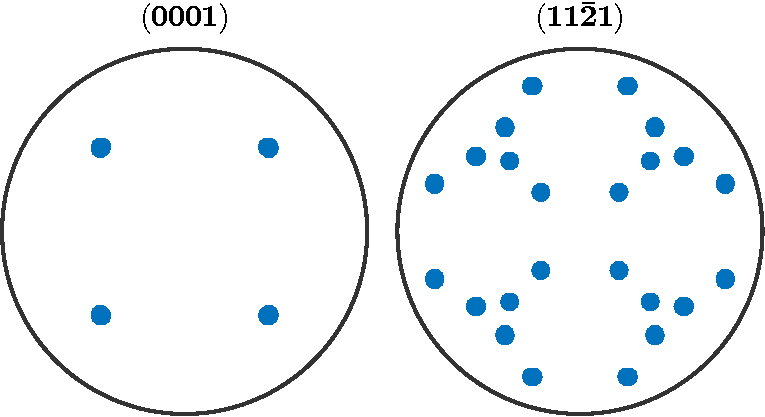
\includegraphics[height=3cm]{pic/HemPDF111.pdf}
    \quad
    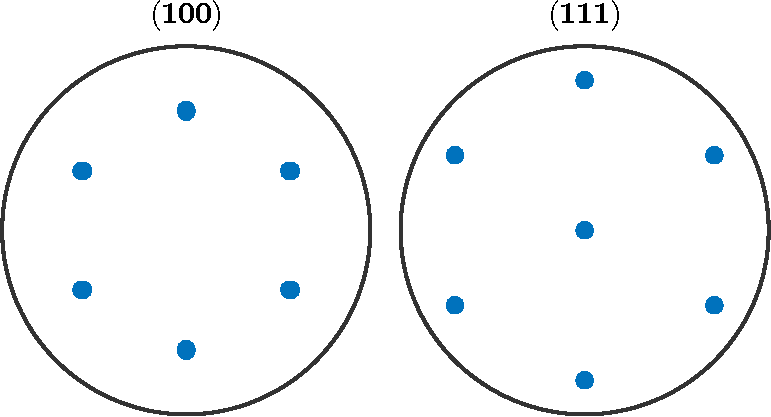
\includegraphics[height=3cm]{pic/MagPDF110.pdf}
  \end{center}
\end{onlyenv}

\end{overlayarea}
\end{frame}

\begin{frame}[fragile]
  \frametitle{Misorientation angel and axis}

  \begin{overlayarea}{\textwidth}{8cm}

    the smallest rotational angle of all symmetrically equivalent
    misorientations to \textbf{MO} is called \structure{misorientation angle}
    \begin{lstlisting}[style=input]
angle(O1,O2) / degree
angle(MO) /degree
    \end{lstlisting}

  \pause
  \medskip

  the misorientation realizing this minimum angle is computed by
  \vspace{-0.2cm}
    \begin{lstlisting}[style=input]
MO.project2FundamentalRegion
    \end{lstlisting}
\begin{onlyenv}<2>
  \vspace{-.3cm}
  \begin{lstlisting}[style=output]
MO = /+misorientation+/ (show methods, plot)
  size: 1 x 1
  crystal symmetry : Magnetite (m-3m)
  crystal symmetry : Hematite (-3m1, X||a*, Y||b, Z||c)

  Bunge Euler angles in degree
     phi1     Phi    phi2    Inv.
  60.1624 54.6037 314.719       0
\end{lstlisting}
\end{onlyenv}

\pause
\medskip

  its rotational axis is called the \structure{misorientation axis} of
  \textbf{MO}
  \vspace{-0.2cm}
\begin{lstlisting}[style=input]
axis(MO)
\end{lstlisting}
\vspace{-.3cm}

  \begin{onlyenv}<3>
\begin{lstlisting}[style=output]
ans = /+Miller+/ (show methods, plot)
 size: 1 x 1
 mineral: Hematite (-3m1, X||a*, Y||b, Z||c)
  h  0.6191
  k  3.8882
  i -4.5073
  l  3.3513
\end{lstlisting}
\end{onlyenv}

  \pause
\begin{lstlisting}[style=input]
axis(inv(MO))
\end{lstlisting}
\vspace{-.3cm}
    \begin{onlyenv}<4>
\begin{lstlisting}[style=output]
ans = /+Miller+/ (show methods, plot)
 size: 1 x 1
 mineral: Magnetite (m-3m)
  h  4.9324
  k -6.4797
  l  2.0431
\end{lstlisting}
\end{onlyenv}

\pause

\begin{lstlisting}[style=input]
axis(O1,O2)
\end{lstlisting}

  \begin{onlyenv}<5>
\vspace{-.3cm}
\begin{lstlisting}[style=output]
ans = /+vector3d+/ (show methods, plot)
 size: 1 x 1
          x         y         z
  0.0495585  0.992437 -0.112305
\end{lstlisting}
\end{onlyenv}

  \end{overlayarea}

\end{frame}


\subsection*{Statistics}

\begin{frame}[fragile]
  \frametitle{Misorientation Statistics}

  \begin{columns}
    \begin{column}{8cm}
      \begin{lstlisting}[style=input]
plotAngleDistribution(MO)
hold on
plotAngleDistribution(MO.CS)
hold off
      \end{lstlisting}

      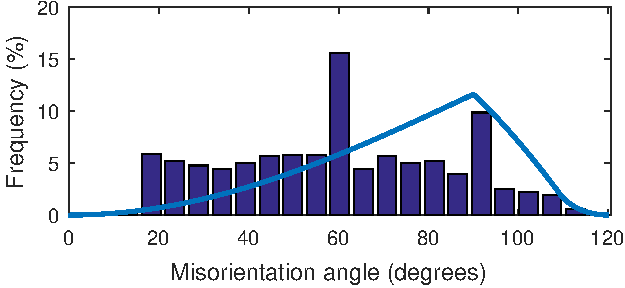
\includegraphics[width=\textwidth]{pic/angleDistri}

      \pause

  \begin{lstlisting}[style=input]
plotAxisDistribution(MO)
  \end{lstlisting}

  \pause
\vspace{-0.3cm}
  \begin{lstlisting}[style=input]
plotAxisDistribution(MO,'contourf')
  \end{lstlisting}
\end{column}
\begin{column}{4cm}
  \begin{overlayarea}{\textwidth}{8cm}
    \begin{onlyenv}<2->
      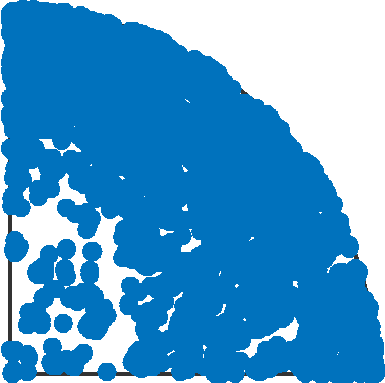
\includegraphics[width = \textwidth]{pic/axisDistri}
    \end{onlyenv}

    \medskip

    \begin{onlyenv}<3>
      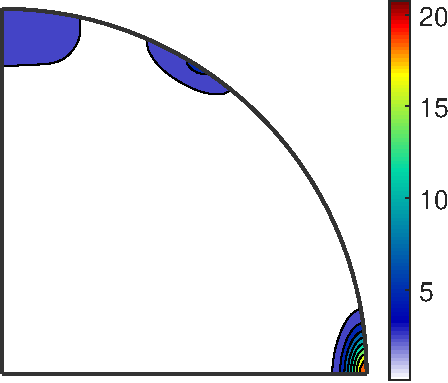
\includegraphics[width = \textwidth]{pic/axisDistriSmooth}
    \end{onlyenv}
  \end{overlayarea}

\end{column}

\end{columns}

\end{frame}


\subsection*{Phase Transitions}


\begin{frame}[fragile]
  \frametitle{Phase Transitions}

  \begin{overlayarea}{\textwidth}{8cm}
    We want to model the phase transition from magnetite to hematite given by
    the orientation relationship $\{111\}_{\text{m}} || \{0001\}_{\text{h}}$
    and $\{\overline{1}01\}_{\text{m}} || \{00\overline{1}0\}_{\text{h}}$
    \begin{lstlisting}[style=input]
CS_Mag = loadCIF('Magnetite')
CS_Hem = loadCIF('Hematite')
   \end{lstlisting}
   \begin{onlyenv}<1>
     \vspace{-0.3cm}
     \begin{lstlisting}[style=output]
cs_Magnetite = /+crystalSymmetry+/ (show methods, plot)
  mineral : Magnetite
  symmetry: m-3m
  a, b, c : 8.4, 8.4, 8.4

cs_Hematite = /+crystalSymmetry+/ (show methods, plot)
  mineral : Hematite
  symmetry : -3m1
  a, b, c : 5, 5, 14
  reference frame: X||a*, Y||b, Z||c
    \end{lstlisting}
  \end{onlyenv}

  \pause
  \medskip

  \begin{lstlisting}[style=input]
Mag2Hem = orientation('map',...
  Miller(1,1,1,CS_Mag),Miller(0,0,0,1,CS_Hem),...
  Miller(-1,0,1,CS_Mag),Miller(1,0,-1,0,CS_Hem),...
  CS_Mag,CS_Hem)
  \end{lstlisting}
  \begin{onlyenv}<2>
    \vspace{-0.3cm}
    \begin{lstlisting}[style=output]
Mag2Hem = /+misorientation+/ (show methods, plot)
  size: 1 x 1
  crystal symmetry : Magnetite (m-3m)
  crystal symmetry : Hematite (-3m1, X||a*, Y||b, Z||c)

  Bunge Euler angles in degree
  phi1 Phi phi2 Inv.
  120 54.7356 45 0
    \end{lstlisting}
  \end{onlyenv}
\end{overlayarea}
\end{frame}


\subsection*{Phase Transition II}

\begin{frame}[fragile]
  \frametitle{Phase Transition}

  \begin{overlayarea}{\textwidth}{8cm}
  For measured hematite orientation
  \begin{lstlisting}[style=input]
ori_Hem = orientation('Euler',0,0,0,CS_Hem)
  \end{lstlisting}
  \begin{onlyenv}<1>
    \vspace{-0.3cm}
    \begin{lstlisting}[style=output]
ori_Hem = /+orientation+/ (show methods, plot)
  size: 1 x 1
  crystal symmetry : Hematite (-3m1, X||a*, Y||b, Z||c)
  specimen symmetry: 1

  Bunge Euler angles in degree
  phi1  Phi phi2 Inv.
     0    0    0    0
    \end{lstlisting}
  \end{onlyenv}
  we can compute the initial magnetite orientation by
  \begin{lstlisting}[style=input]
ori_Mag = ori_Hem * Mag2Hem
  \end{lstlisting}

\pause

  \begin{onlyenv}<2>
    \vspace{-0.3cm}
    \begin{lstlisting}[style=output]
ori_Mag = /+orientation+/ (show methods, plot)
  size: 1 x 1 crystal
  symmetry : Magnetite (m-3m)
  specimen symmetry: 1

  Bunge Euler angles in degree
  phi1 Phi phi2 Inv.
  120 54.7356 45 0
    \end{lstlisting}
  \end{onlyenv}

  \pause
  \medskip

  We should care about symmetric equivalence
  \begin{lstlisting}[style=input]
ori_Mag = ori_Hem * symmetrise(Mag2Hem)
  \end{lstlisting}
  \begin{onlyenv}<3->
    \vspace{-0.3cm}
    \begin{lstlisting}[style=output]
ori_Mag = /+orientation+/ (show methods, plot)
  size: 1 x 96
  crystal symmetry : Magnetite (m-3m)
  specimen symmetry: 1
    \end{lstlisting}
  \end{onlyenv}

\pause

\alert{MTEX keeps track about the symmetries throughout all computations and
  warns in case of mismatch.}
\end{overlayarea}
\end{frame}


\subsection*{phase transistion III}

\begin{frame}[fragile]
  \frametitle{Relationship Between Lattice Planes}

  \begin{overlayarea}{\textwidth}{8cm}

  Compute the minimal angle between two lattice planes of two
  different grains having different orientation and different phase.
 \begin{lstlisting}[style=input]
m_Mag = Miller(1,0,0,cs_Magnetite);
m_Hem = Miller(1,1,-2,0,cs_Hematite);
 \end{lstlisting}
  \begin{onlyenv}<1>
    \vspace{-.3cm}
    \begin{lstlisting}[style=output]
m_Mag = /+Miller+/ (show methods, plot)
 size: 1 x 1
 mineral: Magnetite (432)
  h 1
  k 0
  l 0

m_Hem = Miller (show methods, plot)
 size: 1 x 1
 mineral: Hematite (321, X||a*, Y||b, Z||c)
  h  1
  k  1
  i -2
  l  0
\end{lstlisting}
  \end{onlyenv}

  \pause
  \medskip

  The orientation relation should be given by
  \begin{lstlisting}[style=input]
Mag2Hem = orientation('map',...
  Miller(1,1,1,CS_Mag),Miller(0,0,0,1,CS_Hem),...
  Miller(-1,0,1,CS_Mag),Miller(1,0,-1,0,CS_Hem),...
  CS_Mag,CS_Hem)
  \end{lstlisting}
  \begin{onlyenv}<2>
    \vspace{-0.3cm}
    \begin{lstlisting}[style=output]
Mag2Hem = /+misorientation+/ (show methods, plot)
  size: 1 x 1
  crystal symmetry : Magnetite (m-3m)
  crystal symmetry : Hematite (-3m1, X||a*, Y||b, Z||c)

  Bunge Euler angles in degree
  phi1 Phi phi2 Inv.
  120 54.7356 45 0
    \end{lstlisting}
  \end{onlyenv}

  \pause
  \medskip

  The minimum angle
  \begin{lstlisting}[style=input]
min(angle(Mag2Hem * m_Mag.symmetrise,m_Hem ))/degree
 \end{lstlisting}
  \begin{onlyenv}<3>
    \vspace{-.3cm}
    \begin{lstlisting}[style=output]
  35.2644
    \end{lstlisting}
  \end{onlyenv}

\end{overlayarea}

\end{frame}

% \section{Exercises}

% \subsection*{Exercises2}

% \begin{frame}

%   \begin{Exercise}
%     Consider trigonal crystal symmetry.

%   \begin{enumerate}[a)]
%     \item Find all crystallographic directions symmetrically equivalent to $h
%       = (1, 0, \bar 1, 0)$ (Miller indices)!
%     \item Find crystallographic directions such that the number of their
%       crystallographic equivalent directions on the upper hemisphere (without
%       equator) is 1, 3, and 6, when including antipodal symmetry!
%     \item Consider the orientation given by the Euler angles $(30\degree,
%       90\degree, 90\degree)$ in Bunge convention. Give the Euler angles of
%       all symmetrically equivalent orientations!
%     \item Which positions in the (0,0,0,1) - pole figure corresponds to the
%       above orientation. Which crystal direction is rotated by this
%       orientation to the specimen direction (0,0,1)?
%     \item Construct an orientation that rotates the crystallographic
%       directions $(0,0,0,1)$ and $(2,\bar 1,\bar 1,0)$ onto the specimen
%       directions $(1,0,0)$ and $(0,1,0)$, respectively. Describe the rotation
%       by axis and angle.
%     \end{enumerate}

%   \end{Exercise}

% \end{frame}

\end{document}


% \begin{frame}[fragile]
% \begin{lstlisting}[mathescape=true]
% rot = rotation('Euler',$\phi_1$,$\Phi$,$\phi_2$,'ZXZ')
% rot = rotation('Euler',$\alpha$,$\beta$,$\gamma$,'ABG')
% rot = rotation('axis',v,'angle',omega)
% rot = rotation('map',$u_1$, $v_1$, $u_2$, $v_2$) % $\mathbf{gu}_1=\mathbf{v}_1,\mathbf{gu}_2=\mathbf{v}_2$
% \end{lstlisting}

% \begin{columns}
%   \begin{column}{8.5cm}

%     Calculations:

% \begin{lstlisting}
% v = rot * u    % apply rot to u
% rot = rot1 * rot2
% \end{lstlisting}

%     Basic Functions:

% \begin{lstlisting}[mathescape=true]
% angle(rot), axis(rot)
% angle(rot1,rot2), inv(rot)
% [$\phi_1$,$\Phi$,$\phi_2$] = Euler(rot)
% [$\alpha$,$\beta$,$\gamma$] = Euler(rot,'ABG')
% \end{lstlisting}

%   \end{column}

%   \begin{column}{3cm}
%     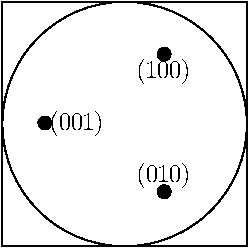
\includegraphics[width=3cm]{pic/quaternion}
%   \end{column}

% \end{columns}
% \end{frame}


% \subsection*{Symmetry}
% \begin{frame}[fragile]
%   \frametitle{Crystal Symmetries - The \MTEX Class \texttt{\bf symmetry}}

%   Definition:

% \begin{lstlisting}
% S = symmetry('triclinic',[a,b,c],[alpha,beta,gamma])
% S = symmetry('-3m',[a,b,c],/+'X||a*'+/);
% S = symmetry('-3m',[a,b,c],'X||a','Z||c*');
% S = symmetry('O');
% \end{lstlisting}

% \medskip

% \begin{columns}
%   \begin{column}{8.5cm}

% Load Symmetry from CIF file:

% \begin{lstlisting}
% symmetry('quartz.cif')
% \end{lstlisting}

% \medskip

%     Basic Functions:

% \begin{lstlisting}
% symmetrise(v,S)
% symmetrise(rot,CS,SS)
% rotation(S)
% project2FundamentalRegion(v,CS)
% project2FundamentalRegion(rot,CS,SS)
% \end{lstlisting}
%   \end{column}

%   \begin{column}{3cm}
%     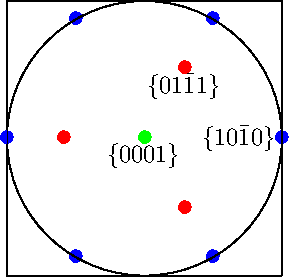
\includegraphics[width=3cm]{pic/sym}
%   \end{column}

% \end{columns}

% \end{frame}

% \subsection*{Miller}

% \begin{frame}[fragile]
%   \frametitle{Crystal Directions - The \MTEX Class \texttt{\bf Miller}}

%   Definition:

% \begin{lstlisting}
% m = Miller(u,v,w,CS,'uvw');
% m = Miller(h,k,i,l,CS,'hkl');
% m = [Miller(1,1,-2,3,CS),Miller(0,1,-1,0,CS)]
% \end{lstlisting}

% \medskip

% \begin{columns}
%   \begin{column}{8.5cm}

%     Calculations:

% \begin{lstlisting}
% h1 + h2
% rot * h     % apply rot on h
% \end{lstlisting}

%     \medskip

%     Basic Functions:

%     \begin{onlyenv}<1>
% \begin{lstlisting}
% eq(h1,h2), angle(h1,h2)
% symmetrise(h)  %get all equivalent
% plot([h1,h2],'all')
% \end{lstlisting}
%     \end{onlyenv}

% 	\end{column}

%   \begin{column}{3cm}
%     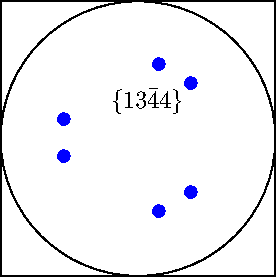
\includegraphics[width=3cm]{pic/miller}
%   \end{column}
% \end{columns}


% 	\begin{onlyenv}<2>

% 		\lstset{stringstyle=\color{red},emph={antipodal},emphstyle=\em\color{red}}

% \begin{lstlisting}
% get(h,'hkl')
% eq(h1,h2,`antipodal`), angle(h1,h2,`antipodal`)
% symmetrise(h,`antipodal`)
% plot([h1,h2],'all',`antipodal`)
% \end{lstlisting}


%     \end{onlyenv}


% \end{frame}



% \begin{frame}[fragile]
%   \frametitle{Orientations - The \MTEX Class \texttt{\bf orientation}}

% Definition:

% \begin{lstlisting}[mathescape=true]
% ori = orientation(rot,CS,SS)
% ori = orientation('Euler',$\phi_1$,$\Phi$,$\phi_2$,CS,SS)
% ori = orientation('Euler',$\alpha$,$\beta$,$\gamma$,'ABG',CS,SS)
% ori = orientation('Miller',[h k l],[u v w],CS,SS)
% ori = orientation('brass',CS,SS)
% \end{lstlisting}

% \begin{columns}
%   \begin{column}{8.5cm}

%     Calculations:

% \begin{lstlisting}
% r = ori * h, h = ori \ r
% ori = rot * ori
% \end{lstlisting}

%     Basic Functions:

% \begin{lstlisting}[mathescape=true]
% eq(ori1,ori2), angle(ori1,ori2)
% symmetrise(ori), angle(ori)
% project2FundamentalRegion(ori,ref_ori)
% [$\phi_1$,$\Phi$,$\phi_2$]  = Euler(ori)
% \end{lstlisting}

%   \end{column}

%   \begin{column}{3cm}
%     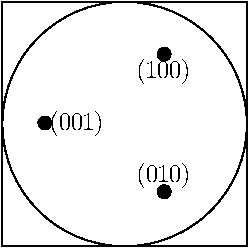
\includegraphics[width=3cm]{pic/quaternion}
%   \end{column}

% \end{columns}
% \end{frame}

2732626
